% Template para Proposta e TCC da EST/UEA -
% Padrão para os cursos do Núcleo de Computação
%
% Elaborado por Elloá B. Guedes
% Adaptado da versão elaborada por:				%                   Jucimar Maia Jr.
%
% Versão beta - 08 de outubro de 2015
%
\documentclass[a4paper,titlepage,12pt]{report}


\usepackage[utf8]{inputenc}
\usepackage[T1]{fontenc}
\usepackage{ae}
\usepackage[brazil]{babel}
\usepackage{a4wide}
\usepackage{comment}
\usepackage[pdftex]{graphicx,color}
\usepackage{graphics}
\usepackage{cite}
\usepackage{longtable}
\usepackage{float}
\usepackage{fancyvrb}
\usepackage{fancyhdr}
\usepackage{setspace}
\usepackage{amsmath}
\usepackage{lscape}
\usepackage{textcase}
\usepackage{anysize}
\usepackage{setspace}
\usepackage{booktabs}
\usepackage{url}
\usepackage{subfig}
\usepackage{cite}
\usepackage[alf]{abntex2cite}

\marginsize{20mm}{20mm}{20mm}{15mm}


%% Cabe�alhos
\renewcommand{\topfraction}{1}
\renewcommand{\bottomfraction}{1}
\renewcommand{\floatpagefraction}{1}
\renewcommand{\textfraction}{0}
%\renewcommand{\baselinestretch}{2}  
\doublespacing %espa�amento duplo
\sloppy

%% Nomes
\floatstyle{plain}  %%% tipos: plain, boxed, ruled
\newfloat{codigo}{tbp}{lop}[section]
\floatname{codigo}{C�digo}

%%% nome para ser usado no sum�rio

\newcommand{\listofcodename}{Lista de C\'{o}digos}



% RESUMO ----------------------------------------------------------------------------------------------------------------------------------------------------------------------

\newcommand{\resumo}[1]{
\begin{center} \LARGE \bf Resumo \end{center} 

\vskip 4em
\input{#1}

\newpage

}

% ABSTRACT ----------------------------------------------------------------------------------------------------------------------------------------------------------------------

\newcommand{\abstractt}[1]{
\begin{center} \LARGE \bf Abstract \end{center} 

\vskip 4em
\input{#1}

\newpage

}

% Sum�rio -----------
\newcommand{\sumario}{
\renewcommand{\contentsname}{Sum\'{a}rio}
\tableofcontents
\addcontentsline{toc}{chapter}{\listtablename}
\listoftables

\newpage
\addcontentsline{toc}{chapter}{\listfigurename}
\listoffigures
\addcontentsline{toc}{chapter}{\listofcodename}
\listof{codigo}{\listofcodename}  % Lista de C�digos

\clearpage
}



\pagestyle{plain}

\newcommand{\folhaRosto}[5]{

\thispagestyle{empty}
\begin{center}
\textbf{\\[0.4em]\MakeUppercase{#2} \\[5cm]}
\textbf{\MakeUppercase{#1}\\[96pt]}

\end{center}

\hspace*{8cm}
\begin{minipage}{8cm} 
Trabalho de Conclusão de Curso
apresentado à banca avaliadora do Curso de Engenharia de Computação, da 
Escola Superior de Tecnologia, da Universidade do Estado do Amazonas, como
pré-requisito para obtenção do título de Engenheiro de Computação.\\[40pt] 
\end{minipage} 

\begin{center}
Orientador(a): #3 \\[12ex]
Manaus -- #4 -- #5\\
\end{center}


\pagenumbering{roman}
\newpage
}



%% Preencha aqui os seguintes dados
\def \titulo{Uma Plataforma Web para Gerenciamento de Dados e Geração de Boletins Meteorológicos do LabInstru}
\def \orientador{Profa. Dra. Elloá Barreto Guedes da Costa}
\def \nome{Pedro Augusto Franco Ribeiro}
\def \mes{Novembro}
\def \ano{2017}

\begin{document}

\folhaRosto{\titulo}{\nome}{\orientador}{\mes}{\ano}

% Edite os seguintes arquivos para alterar as informações necessárias
% ficha Catalográfica------------------------------------------------------------------------------------------------------------------------------------------
\begin{spacing}{1.4}
\textit{\textbf{\\
Universidade do Estado do Amazonas - UEA\\
Escola Superior de Tecnologia - EST}}

\textit{\\
Reitor:\\ 
\textbf{
Carlos Eduardo de Souza Gonçalves}\\
Vice-Reitor:\\ \textbf{Nome do Vice-Reitor}}
\\
\textit{
Diretor da Escola Superior de Tecnologia:\\ 
\textbf{Mário Augusto Bessa de Figueirêdo}}
\\
\textit{
Coordenador do Curso de Engenharia de Computação:\\
\textbf{Antenor Ferreira Filho}}
\\
\textit{
Coordenador da Disciplina Projeto Final:\\
\textbf{Jucimar Maia da Silva Júnior}}
\\[12pt]
\textit{
Banca Avaliadora composta por: \hfill Data da Defesa:  /  /2015.\\
}
\textit{ 
\textbf{Profa. Dra. Elloá Barreto Guedes da Costa} (Orientador(a))\\
\textbf{Prof. M.Sc. }\\% Escreva o nome dos professor da sua banca antes de '\\' (comando para quebra de linha)
\textbf{Prof. M.Sc. }
}
\center{\bf CIP -- Catalogação na Publicação}\ \ \\
 \begin{small}
\begin{center}
\fbox{
\parbox{18cm}{
\begin{minipage}{17cm} 
L864a \hspace*{1cm} MARINHO, Deyvid Eric de Moraes\\[12pt]
\hspace*{2cm} \parbox{14cm}{
\hspace*{0.5cm}Desenvolvimento de Padrão para Monografias de Engenharia de Computação da UEA / 
Lanier Santos; [orientado por] Profa. Dra. Elloá Barreto Guedes da Costa -- Manaus: UEA, 2015.\\
\hspace*{0.5cm}240 p.: il.; 30cm\\
\hspace*{0.5cm}Inclui Bibliografia\\
\hspace*{0.5cm}Trabalho de Conclusão de Curso (Graduação em Engenharia de Computação).
Universidade do Estado do Amazonas, 2015.\\[6pt]
\hspace*{8cm} CDU: \hrulefill}
\end{minipage}}}
\end{center}
\end{small}
\end{spacing}
 \newpage

% folha de aprovação----------------------------------------------------------------------------------------------------------------------------------

\begin{center}
\bf \MakeUppercase{\nome}\\[1.5 cm]
\end{center}

\begin{center}
\bf \MakeUppercase{\titulo}\\[1.5cm]
\end{center}

\hspace*{8cm}
\begin{minipage}{8cm}

Trabalho de Conclusão de Curso apresentado à
banca avaliadora do Curso de Engenharia de Computação,
da Escola Superior de Tecnologia, da Universidade do Estado do Amazonas,
como pré-requisito para obtenção do título de
Engenheiro de Computação.\\

\large \bf Aprovado em: 05/12/2017
\end{minipage}

BANCA EXAMINADORA\\[12 pt]

\noindent \hrulefill \hspace*{6cm} \\
\noindent \textbf{\orientador}\\
\textit{UNIVERSIDADE DO ESTADO DO AMAZONAS}\\[0.5cm]

\noindent \hrulefill \hspace*{6cm} \\
\noindent \textbf{Profa. Márcia Sampaio Lima, M.Sc.}\\
\textit{UNIVERSIDADE DO ESTADO DO AMAZONAS}\\[0.5cm]

\noindent \hrulefill \hspace*{6cm} \\
\noindent \textbf{Prof. Flávio José Coelho, M.Sc.}\\
\textit{UNIVERSIDADE DO ESTADO DO AMAZONAS}\\



% Indique onde esta o arquivo do resumo
\resumo{./files/resumo.tex}
% Idem para o abstract
\abstractt{./files/abstract.tex}


\sumario

% Configuração de cabeçalhos
\pagestyle{fancy}
\renewcommand{\chaptermark}[1]{\markboth{#1}{}}
\renewcommand{\sectionmark}[1]{\markright{#1}}
\renewcommand{\headrulewidth}{0.5pt}
\newcommand{\rom}{\fontfamily{cmr}\fontseries{m}\fontsize{10}{12}\selectfont}
\fancyhf{} \fancyhead[LE,RO]{\rom\thepage}
\fancyhead[LO]{\rom\rightmark} \fancyhead[RE]{\rom\leftmark}
\fancypagestyle{plain}{
    \fancyhead{} % get rid of headers
    \renewcommand{\headrulewidth}{0pt} % and the line
 }


\pagenumbering{arabic} 


% Seus capítulos vão aqui --------
\chapter{Introdução}

As tecnologias computacionais relacionadas ao processamento de dados permitem uma melhor forma de manusear uma grande quantidade de informação. Se determinados processamentos fossem realizados manualmente, a quantidade de tempo necessária poderia inviabilizar a sua realização. Além disso, os eventuais resultados também poderiam estar sujeitos à erros de manipulação, os quais seriam difíceis de detectar. Considerado estas dificuldades, diversas áreas do cotidiano utilizam a tecnologia como uma aliada, por exemplo a Meteorologia, responsável pelo estudo do clima e das condições de tempo de uma determinada região.

Algumas das atribuições da Meteorologia compreendem o entendimento do estado presente da atmosfera, o chamado ``tempo meteorológico'', e a realização de previsões, a chamada ``previsão do tempo'' \cite{Vianello:Livro}. No caso do tempo meteorológico, se faz necessário medidas de diferentes variáveis como temperatura do ar, umidade relativa do ar, direção e velocidade do vento, precipitação, pressão atmosférica, radiação, dentre outras. Considerando o grande volume de dados comum a este domínio, é essencial que tecnologias, métodos e ferramentas auxiliem a realização dessas tarefas propostas.

Visando um melhor entendimento das questões meteorológicas de Manaus e da Amazônia, em março de 2010 foi fundado o \emph{Laboratório de Instrumentação Meteorológica} (LabInstru) da Escola Superior de Tecnologia (EST) da Universidade do Estado do Amazonas (UEA). Este laboratório dispõe, dentre outros, de uma estação meteorológica automática, localizada nas dependências da EST/UEA, sob as coordenadas \ang{03;05;32,5}S, \ang{60;00;59,69}W a 31 metros acima do nível do mar, na qual diversos sensores encontram-se instalados para medida e registros de diferentes variáveis meteorológicas \cite{Labinstru:EST}.

Além da manutenção da estação meteorológica, o LabInstru possui uma série de atribuições, tais como a organização dos dados coletados, disponibilização de dados para órgãos governamentais e para a sociedade, geração de boletins meteorológicos informativos, dentre outros. Atualmente, a maioria dessas atividades têm sido realizada de forma manual, um processo demorado e exaustivo, sujeito a erros e imprecisões e que requer mão de obra altamente especializada.

Para ilustrar o contexto considerado, um exemplo é apresentado na Figura \ref{fig:contexto}. Se um interessado desejar adquirir uma determinada informação, primeiramente deverá preencher um formulário online disponível no site do LabInstru e também entregar, presencialmente no próprio laboratório, o termo de compromisso adequado à sua solicitação devidamente preenchido (Etapa 1). Em seguida, a equipe do laboratório recebe uma notificação da solicitação (via e-mail) e inicia a preparação dos dados (Etapa 2). O passo seguinte consiste em consultar diferentes arquivos-texto resultantes da estação meteorológica a fim de precisar o intervalo de datas requerido (Etapa 3). A equipe irá agregar esses dados e utilizará aplicativos adequados para filtrar as variáveis meteorológicas requeridas pela solicitação (Etapa 4).

\begin{figure}[H]
	\centering
	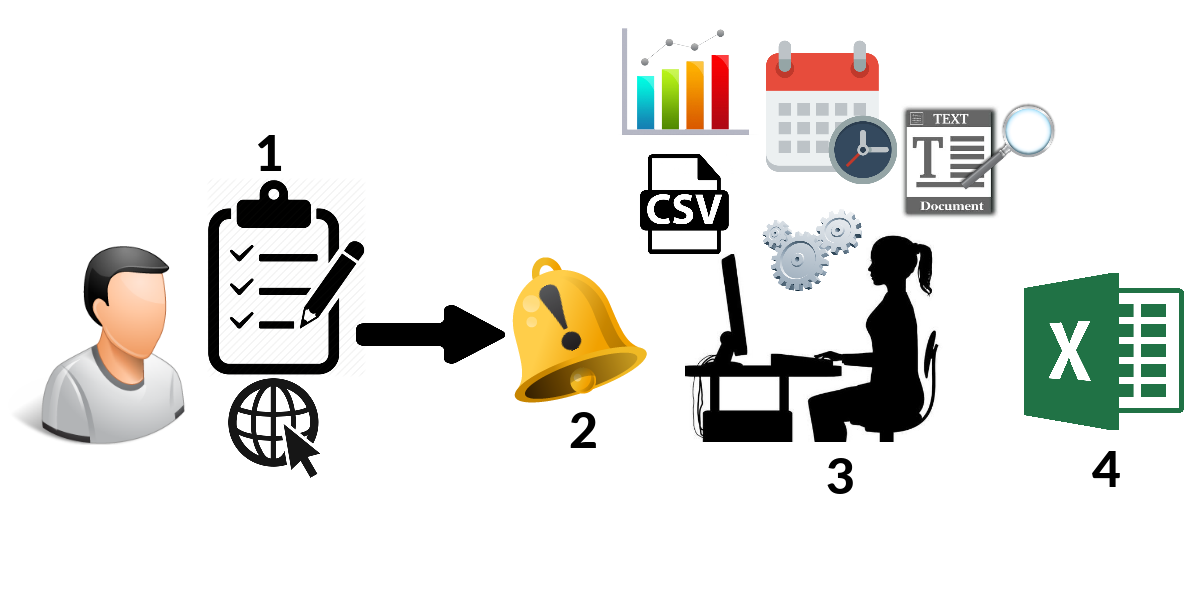
\includegraphics[width=0.6\textwidth]{./img/contexto.png}
	\caption{Contexto atual de uma das atividades realizadas pelo LabInstru. Fonte: Próprio Autor} 			\label{fig:contexto}
\end{figure}

Embora este exemplo ilustre o cenário atual do LabInstru, não compreende todas as dificuldades enfrentadas pela equipe do laboratório na realização de suas atribuições. Há que se mencionar as dificuldades na preparação de gráficos ilustrativos, na verificação da disponibilidade de dados, na geração de boletins meteorológicos, no controle e manuseio dos arquivos da estação meteorológica, dentre diversas outras.

Considerando este contexto, este trabalho de conclusão de curso teve por objetivo projetar e implementar uma plataforma web com vistas a colaborar na minimização das dificuldades mencionadas. Para tanto, contemplou o armazenamento, gerenciamento e disponibilização de dados da estação meteorológica automática da EST/UEA, administrada pelo LabInstru, fornecendo também uma visualização desses dados por meio de boletins meteorológicos.

\todo{Falta aqui uma visão geral sobre o que foi feito.}

\section{Objetivos}

O objetivo geral deste trabalho consistiu projetar e implementar uma plataforma web, para armazenamento, gerenciamento e disponibilização de dados de uma estação meteorológica automática. Para obtenção de sucesso no objetivo apresentado, fez-se necessário alcançar alguns objetivos específicos, a citar:

\begin{enumerate}
	\item Identificar e documentar as funcionalidades que a plataforma a ser desenvolvida deve prover;
	\item Elaborar protótipos de interface para validar as funcionalidades a serem desenvolvidas;
	\item Efetuar um levantamento das tecnologias para o desenvolvimento da plataforma web;
	\item Projetar e implementar a plataforma web;
	\item Implantar a plataforma web no LabInstru.
\end{enumerate}

\section{Justificativa}

O desenvolvimento de uma plataforma web para o LabInstru é importante por diversas razões. Primeiramente sabe-se que a forma como os dados meteorológicos são armazenados e as técnicas utilizadas para processamento influenciam diretamente na precisão e no tempo gasto para a realização de diversas tarefas. Assim, o desenvolvimento de uma plataforma para este domínio colabora diretamente na minimização destas dificuldades, visto que se propõe a  armazenar, gerenciar e disponibilizar os dados de maneira estruturada e automatizada.

Esta plataforma colabora de maneira direta com uma das atividades centrais do LabInstru, que compreende a organização dos dados coletados na estação instalada através do laboratório \cite{Labinstru:EST}. Há que se mencionar também que uma plataforma desta natureza favorece a divulgação dos dados meteorológicos produzidos. Estes são de interesse para pesquisadores de diversas áreas, para autoridades governamentais e também para a população em geral, como é amplamente visto na mídia.

Do ponto de vista da Engenharia de Computação, este trabalho de conclusão de curso também colabora com métodos e técnicas desta área do conhecimento aplicadas ao domínio da Meteorologia, auxiliando no desenvolvimento de uma plataforma que será usada em contexto real, por usuários reais e que irá colaborar para a manutenção de um laboratório de pesquisas de uma instituição pública de ensino superior, fomentando a realização de diversos outros trabalhos.

\section{Metodologia} \label{sec:metodologia}

A metodologia adotada para guiar as atividades deste trabalho de conclusão de curso é apresentada a seguir, a qual compreendeu a realização das seguintes atividades:

\begin{enumerate}[label=\textbf{Atividade \arabic*}.,leftmargin=*,labelindent=1em]
	\item Identificar um processo de desenvolvimento que possa acomodar as características do trabalho em questão, considerando que novos requisitos podem ser descobertos, que só há um desenvolvedor e que não deve haver \emph{overhead} na documentação das atividades;
	\item Estudo dos arquivos gerados pela estação meteorológica do LabInstru, pré-requisito para o entendimento de diversos requisitos;
	\item Efetuar a elicitação de requisitos funcionais e não funcionais referentes ao domínio do problema, construindo diagramas de caso de uso e documentando os requisitos descobertos apropriadamente;
	\item Utilizando uma ferramenta de \emph{mockups}, construir protótipos da interface gráfica que permitam validar junto ao cliente os requisitos identificados;
	\item Elencar uma ordem de implementação dos requisitos considerando as dependências entre os mesmos e o cronograma disponível do trabalho de conclusão de curso;
	\item Identificar tecnologias para o desenvolvimento da plataforma web, considerando \emph{frameworks} que possam ajudar nesta tarefa e também recursos que possam auxiliar no desenvolvimento do \emph{front-end}, permitindo a criação da interface gráfica com recursos que venham a prover uma boa usabilidade;
	\item Implementar os requisitos considerando a ordem anteriormente especificada;
	\item Escrever o trabalho de conclusão de curso I;
	\item Defesa do trabalho de conclusão de curso I;
	\item Implantar a plataforma web junto ao cliente, permitindo a utilização da mesma pelos pesquisadores do LabInstru. Avaliar a possibilidade de instalação em um servidor local ou hospedagem em um servidor externo;
	\item Escrever o trabalho de conclusão de curso II;
	\item Defesa do trabalho de conclusão de curso II.
\end{enumerate}

\section{Organização do Documento}

Para apresentar a solução proposta, este trabalho de conclusão de curso está organizado como segue. O Capítulo \ref{cap:fundamentacao} apresenta os conceitos essenciais que foram utilizados no desenvolvimento deste trabalho, incluindo o contexto da Estação Meteorológica da EST, o boletim meteorológico do LabInstru e conceitos da Meteorologia, tais como índice de calor e escala de Beaufort. O Capítulo \ref{cap:solucao} apresenta a solução proposta, contemplando desde uma visão geral da mesma, os artefatos de modelagem produzidos, protótipos e a versão executável da mesma implementada na linguagem de programação Python, com o \emph{framework} Web2py. Por fim, as considerações finais e sugestões de trabalhos futuros encontram-se descritos no Capítulo \ref{cap:consideracoes}.

\chapter{Fundamentação Teórica}
\chapter{Solução Proposta} \label{cap:solucao}

Em resposta aos problemas identificados para processar as informações geradas pela estação meteorológica da EST e geração dos boletins meteorológicos, este trabalho se propôs a projetar e implementar uma plataforma web para gerenciamento de dados e geração de boletins meteorológicos do LabInstru. As seções a seguir apresentam artefatos resultantes da análise do problema e da concepção da solução proposta, detalhando os elementos que a caracterizam.


\section{Processo de Desenvolvimento Adotado}
O AUP foi escolhido como modelo de processo de desenvolvimento por seguir a metodologia ágil e por possuir diversos elementos que capturam a realidade do contexto em que este trabalho de conclusão de curso está sendo desenvolvido. Além dos elementos mencionados, um outro fator prepoderante para escolha do AUP foi o fato do software  desenvolvido não ser de grande porte e possuir uma equipe pequena de desenvolvimento, nesse caso, composta apenas de uma pessoa -- o aluno.

A Profa. Maria Betânia Leal exerceu o papel de cliente final da aplicação. O papel de solicitante do software foi exercido pela Profa. Elloá B. Guedes, a qual forneceu \emph{feedback} e auxiliou na validação das funcionalidades desenvolvidas.

Por estar baseado em uma abordagem iterativa e incremental, o AUP auxiliou a organização deste trabalho em séries de pequenas iterações, que puderam ser efetuadas levando em consideração um caso de uso por vez. Desta maneira, teve-se sempre um sistema parcial executável e testável, em que as partes desenvolvidas puderam ser facilmente integradas.

Em relação à algumas disciplinas do AUP, algumas decisões foram consideradas. Em termos de testes, foram considerados os testes feitos pelo próprio desenvolvedor utilizando os recursos disponíveis na linguagem de programação adotada, tal como o comando \texttt{assert}. O gerenciamento de configuração será efetuado com o auxílio das ferramentas Google Drive e Git para gerenciamento de documentos e de código, respectivamente. A disciplina de gerenciamento de projetos foi liderada pela profa. Elloá B. Guedes, que promoveu reuniões com a cliente sempre que necessário e estabeleceu prazos, atividades e marcos de entrega de acordo com o planejamento semestral do trabalho de conclusão de curso.


\section{Diagramas de Caso de Uso}
Após conversas com a cliente e com a solicitante do software, foi possível identificar quatro módulos principais que contemplam as diferentes funcionalidades solicitadas. Estes módulos são apresentados a seguir:

\begin{enumerate}
	\item \textbf{Módulo Gerencia Conta de Usuário}. Neste módulo, cujo ator principal é o administrador do sistema, concentram-se as funcionalidades relativas à manutenção de usuários, ilustradas no diagrama de caso de uso da Figura \ref{fig:casoUso1}. No cenário em que a plataforma será utilizada, foi possível identificar que não deve haver livre cadastro e acesso aos dados de maneira deliberada, daí a necessidade de um administrador para cadastrar novos usuários, que podem ser alunos de iniciação científica, pesquisadores, docentes, dentre outros;
	\begin{figure}[H]
		\centering
		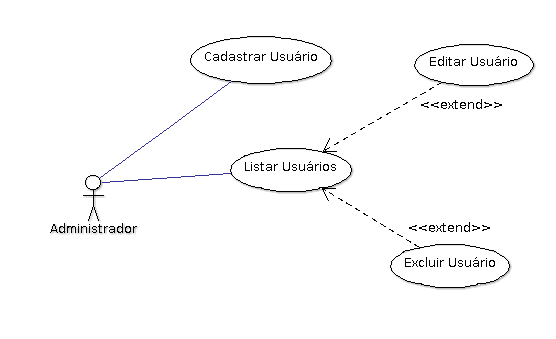
\includegraphics[scale=0.8]{img/uc001.png}
		\caption{Caso de Uso - Módulo Gerencia Conta de Usuário.}
		\label{fig:casoUso1}
	\end{figure}
	\item \textbf{Módulo Usuário}. Neste módulo, cujo ator principal é o usuário, encontram-se as funcionalidades relativas à manutenção dos dados do próprio usuário. Pode haver alterações de dados do perfil, redefinição e recuperação de senha, conforme ilustrado na Figura \ref{fig:casoUso2};
	\begin{figure}[H]
		\centering
		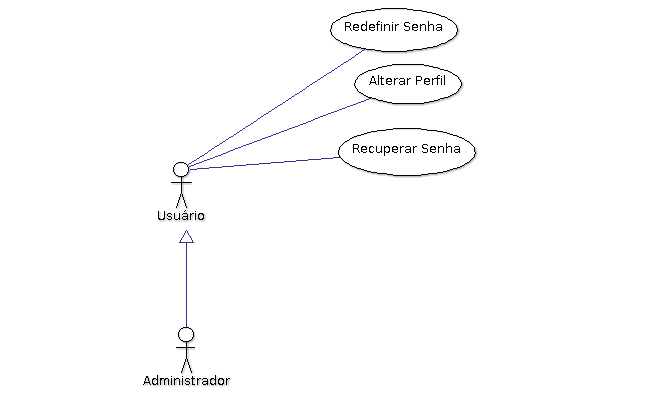
\includegraphics[scale=0.8]{img/uc002.png}
		\caption{Caso de Uso - Módulo Usuário.}
		\label{fig:casoUso2}
	\end{figure}
	\item \textbf{Módulo Consulta Medições}. Este módulo concentra as funcionalidades de acesso aos dados das estações. Conforme ilustra a Figura \ref{fig:casoUso3}, podem ser feitas consultas diretas aos dados, consulta à disponibilidade dos dados em um determinado mês e também aspectos da visualização dos dados, seja por meio de boletins como também por meio de gráficos, além da possibilidade de exportação. Estas funcionalidades foram identificadas considerando as principais solicitações de dados feitas por terceiros ao LabInstru;
	% figura 3
	\begin{figure}[H]
		\centering
		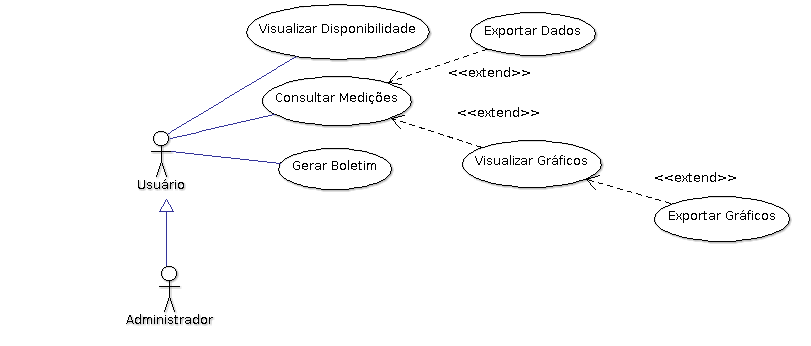
\includegraphics[scale=0.8]{img/uc003.png}
		\caption{Caso de Uso - Módulo Consulta Medições.}
		\label{fig:casoUso3}
	\end{figure}
	\item \textbf{Módulo Gerencia Medições}. O módulo de gerenciamento de medições permite que o administrador do sistema mantenha as medições do sistema a partir dos dados obtidos das estações meteorológicas do LabInstru. Considerando a importância de assegurar a origem destes dados e a remoção das eventuais medições inconsistentes, apenas o administrador está habilitado para execução das funcionalidades deste módulo, conforme ilustrado na Figura \ref{fig:casoUso4}.
	% figura 4
	\begin{figure}[H]
		\centering
		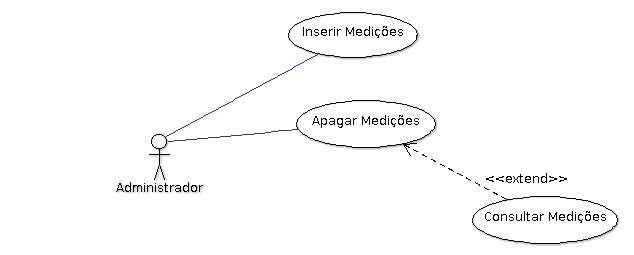
\includegraphics[scale=0.8]{img/uc004.png}
		\caption{Caso de Uso - Módulo Gerencia Medições.}
		\label{fig:casoUso4}
	\end{figure}
\end{enumerate}

O detalhamento de todos os casos de uso ilustrados nas Figuras \ref{fig:casoUso1}-\ref{fig:casoUso4} encontra-se disponível no Apêndice \ref{sec:aprendiceCasoUso},  onde podem ser vistos os interessados, pré e pós condições, fluxo principal, fluxo alternativo e regras de negócio.


\section{Prototipação das Telas do Usuário}
Considerando as funcionalidades identificadas e documentadas, partiu-se para elaboração de protótipos. Estes protótipos foram construidos considerando as principais funcionalidades a serem desenvolvidas, com o intuito de mostrar à cliente uma representação limitada da solução proposta, mas que permitisse explorar a sua conveniência. O resultado desta prototipação é mostrado a seguir. Embora os protótipos de todas as funcionalidades tenham sido elaborados, apenas os mais relevantes serão mostrados a seguir. Para elaborá-los foi utilizado o software Balsamiq Mockups \cite{Prototipacao:Mockups}.

A tela inicial da aplicação encontra-se ilustrada na Figura  \ref{fig:tela002}. No canto superior direito, há um link para o formulário de autenticação no sistema e também para recuperação de senha, caso algum usuário tenha esquecido da mesma.

\begin{figure}[H]
	\centering
	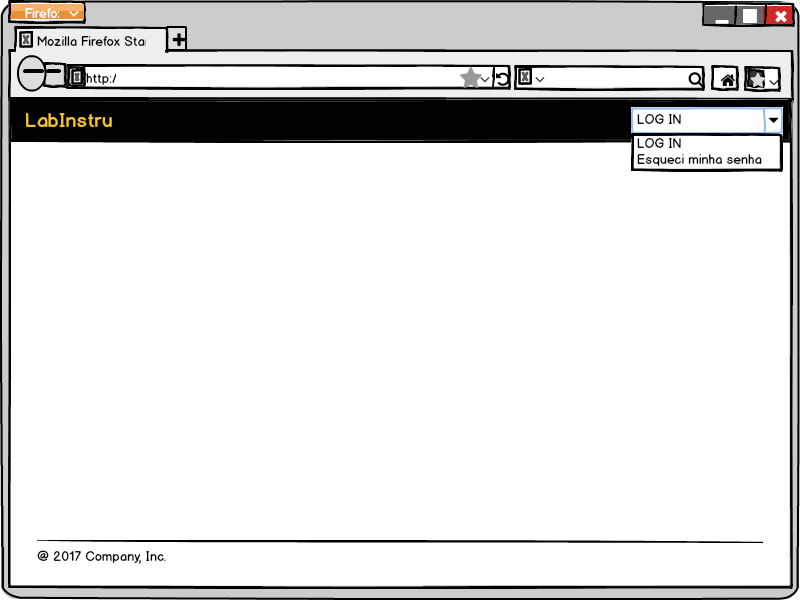
\includegraphics[width=0.8\textwidth]{./img/telas/tela002.png}
	\caption{Tela inicial da aplicação web LabInstru.} \label{fig:tela002}
\end{figure}

Considerando a perspectiva do usuário Administrador, o menu principal da aplicação disponível para o mesmo é mostrado na Figura \ref{fig:tela025}, no qual é possível selecionar a opção ``Cadastrar Usuário'' na aba ``Administração''.  Para efetuar a inclusão de um novo usuário na base de dados, o administrador será redirecionado para o formulário de cadastro ilustrado na Figura \ref{fig:tela027}.


\begin{figure}[H]
	\centering
	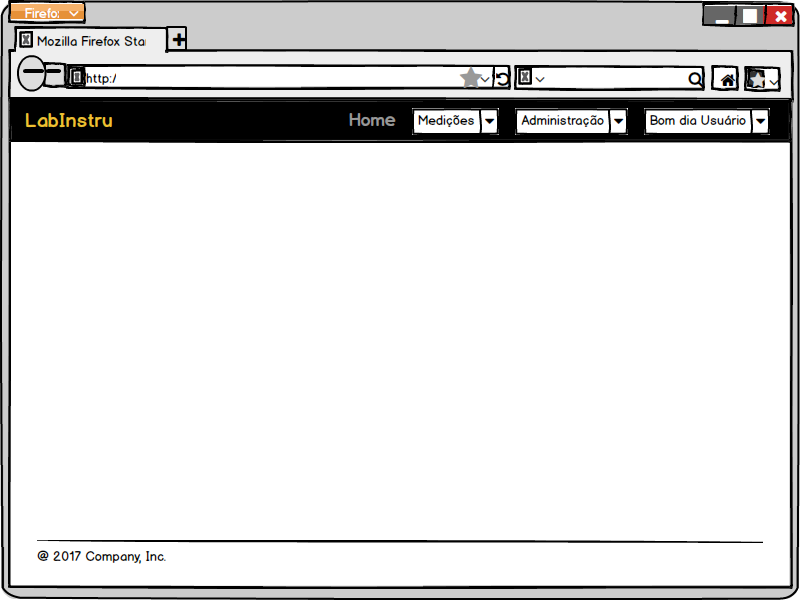
\includegraphics[width=0.8\textwidth]{./img/telas/tela025.png}
	\caption{Protótipo de tela do menu principal da aplicação.} \label{fig:tela025}
\end{figure}


\begin{figure}[H]
	\centering
	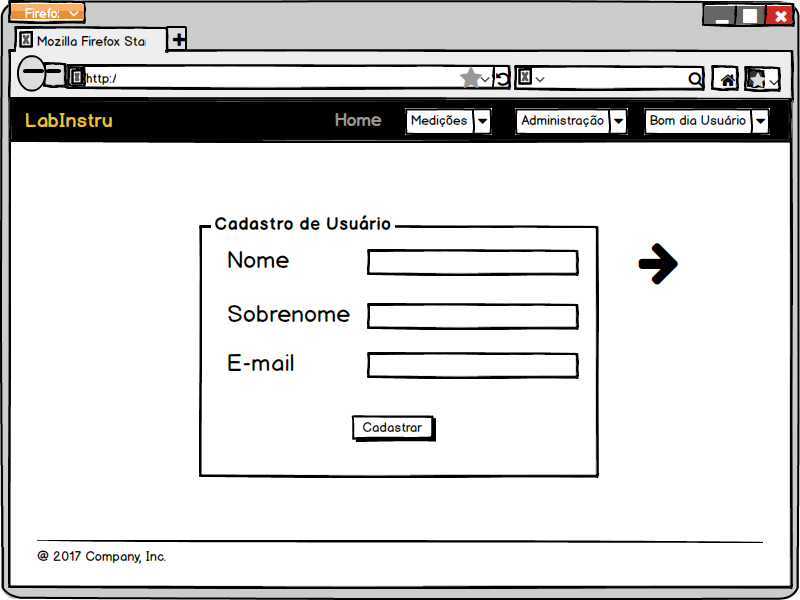
\includegraphics[width=0.8\textwidth]{./img/telas/tela027.png}
	\caption{Protótipo de tela referente ao cadastrado de usuário.} \label{fig:tela027}
\end{figure}

Para exibe uma listagem dos usuários cadastrados na base de dados da aplicação, e posteriormente, caso desejável, fazer a edição ou remoção de um usuário específico, deve-se esoclher a opção ``Listar Usuários'' na aba ``Administração'' do menu principal da aplicação, conforme Figura \ref{fig:tela033}.

\begin{figure}[H]
	\centering
	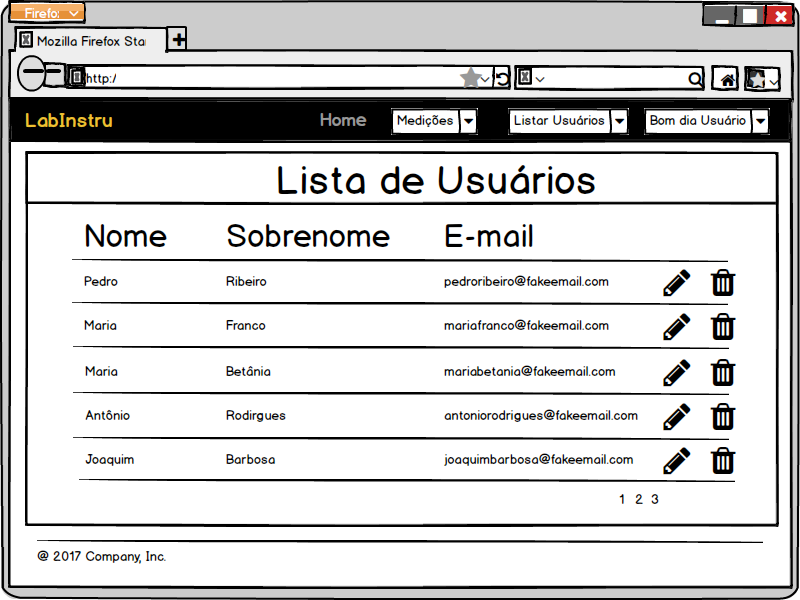
\includegraphics[width=0.8\textwidth]{./img/telas/tela033.png}
	\caption{Protótipo de tela referente à listagem de usuários.} \label{fig:tela033}
\end{figure}

O cadastro de novas medições é efetuado pelo Administrador. Para tanto, este deve utilizar um formulário análogo ao mostrado na Figura \ref{fig:tela053}, em que este deve fornecer um arquivo oriundo da estação meteorológia no formato \texttt{.dat}.

\begin{figure}[H]
	\centering
	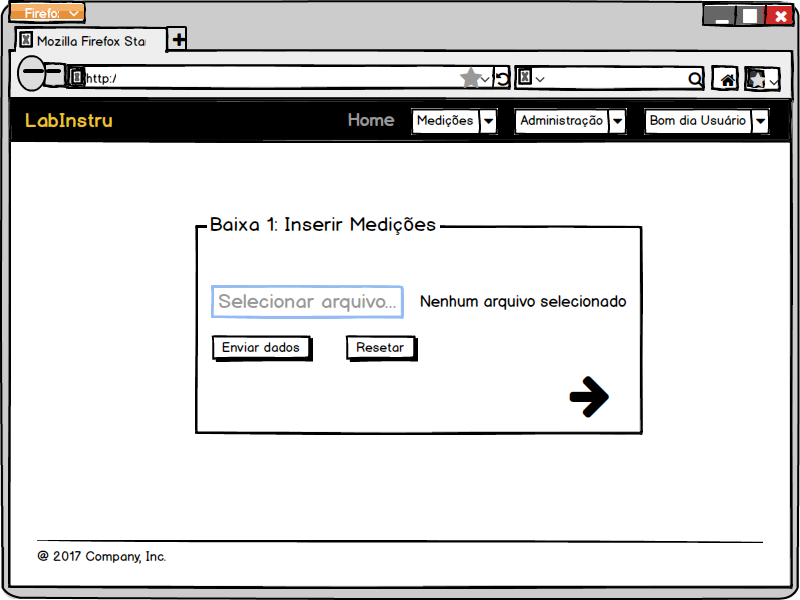
\includegraphics[width=0.8\textwidth]{./img/telas/tela053.png}
	\caption{Protótipo de tela para cadastro de novas medições.} \label{fig:tela053}
\end{figure}

Caso um usuário deseje efetuar uma consulta na base de dados, um formulário detalhado será exibido, conforme ilustrado na Figura  \ref{fig:tela058}, no qual o usuário deve informar os parâmetros para consulta dos dados. Ao submeter a consulta, as respostas serão exibidas conforme ilustrado na Figura \ref{fig:tela062}.

\begin{figure}[H]
	\centering
	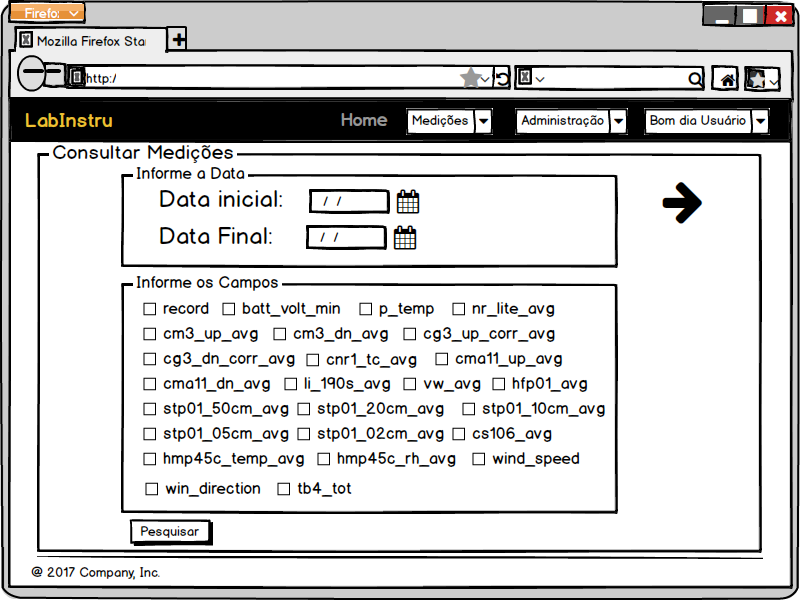
\includegraphics[width=0.8\textwidth]{./img/telas/tela058.png}
	\caption{Protótipo de tela referente ao formulário para consultar medições.} \label{fig:tela058}
\end{figure}

\begin{figure}[H]
	\centering
	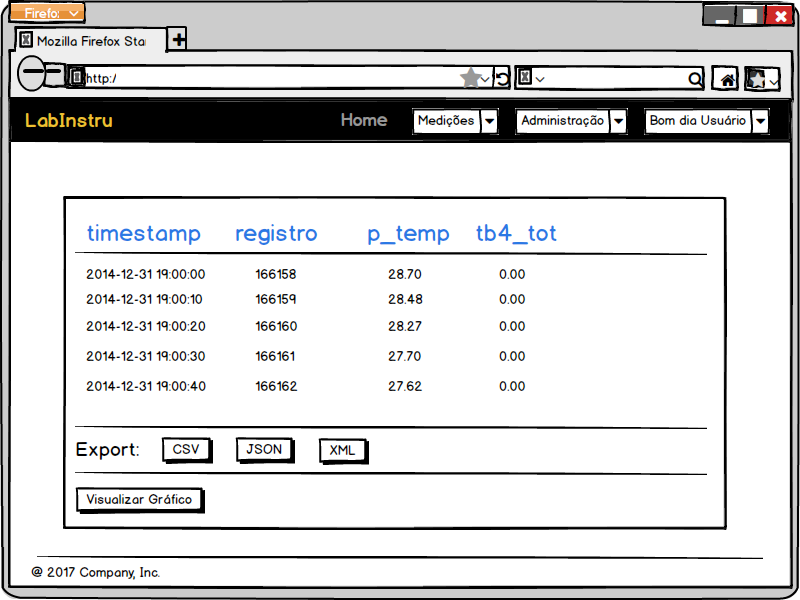
\includegraphics[width=0.8\textwidth]{./img/telas/tela062.png}
	\caption{Protótipo de tela referente à visão de saída a uma consulta de medições.} \label{fig:tela062}
\end{figure}

Por meio do menu principal da aplicação, escolhendo a opção disponibilidade, pertecente à aba de uma determinada estação meteorológica (Baixa 1 ou Baixa 2), vide Figura \ref{fig:tela072}, é possível ter acesso ao calendário de disponibilidade de medições diárias desta estação meteorológica. Esse calendário, conforme ilustrado na Figura \ref{fig:tela073}, tem por objetivo informar quantas medições estão disponíveis em todos os dias do mês escolhido, por meio de cores apropriadas.

\begin{figure}[H]
	\centering
	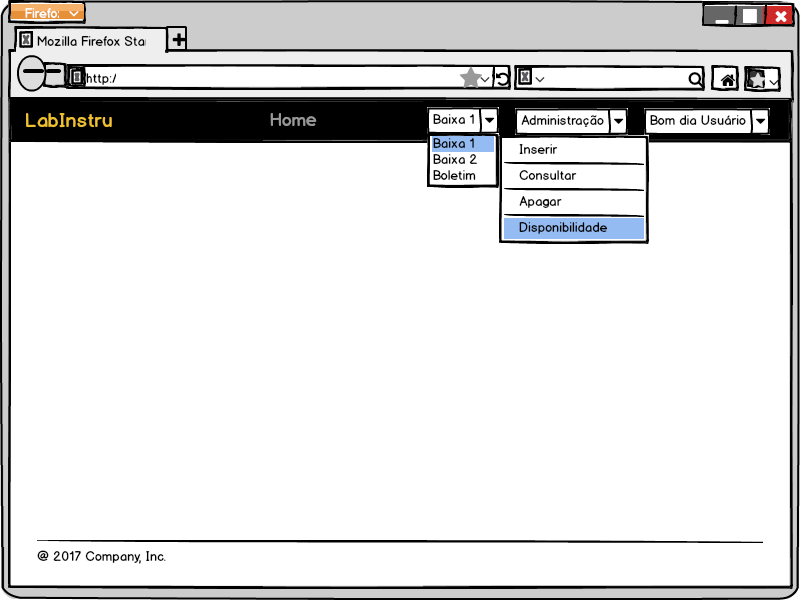
\includegraphics[width=0.8\textwidth]{./img/telas/tela072.png}
	\caption{Navegando no menu para funcionalidade Disponibilidade.} \label{fig:tela072}
\end{figure}

\begin{figure}[H]
	\centering
	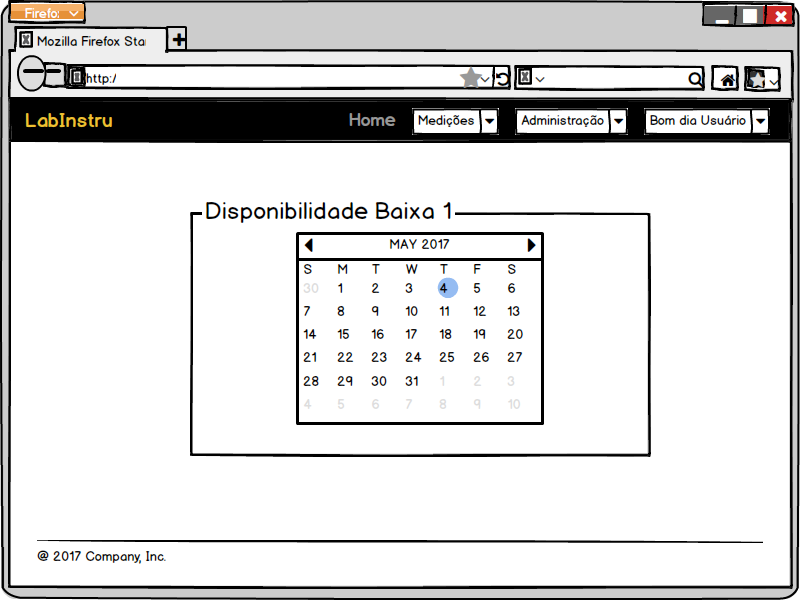
\includegraphics[width=0.8\textwidth]{./img/telas/tela073.png}
	\caption{Tela responsável por exibir o calendário de disponibilidade.} \label{fig:tela073}
\end{figure}

Outra funcionalidade importante na aplicação é o \textit{Boletim Meteorológico}, que pode ser acessado por meio da opção \textit{``Boletim''}, na aba \textit{``Medições''} do menu principal da aplicação. Esse boletim informará diversos dados meteorológicos (temperatura máxima, mínima, índice de calor, etc.) por dia de um determinado mês. A Figura \ref{fig:tela077} ilustra um exemplo de processamento resultante desta funcionalidade.

\begin{figure}[H]
	\centering
	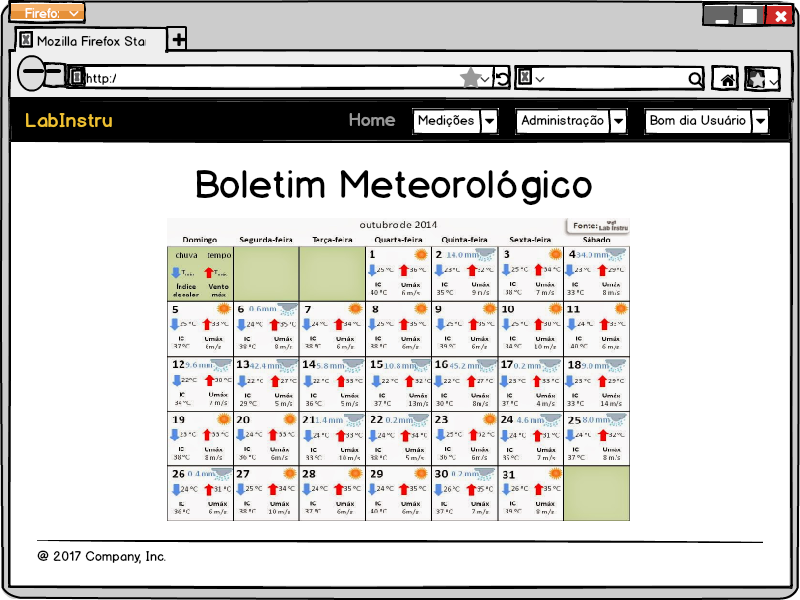
\includegraphics[width=0.8\textwidth]{./img/telas/tela077.png}
	\caption{Protótipo de tela responsável por mostrar o resultado do boletim meteorológico.} \label{fig:tela077}
\end{figure}


\section{Tecnologias Utilizadas}
As tecnologias utilizadas para elaboração da solução proposta consistem no \emph{framework} Web2py, detalhado anteriormente na Seção \ref{sec:web2py}, nos \emph{frameworks} Bootstrap, na biblioteca JQuery e no sistema gerenciador de banco de dados MySQL. Uma visão geral de cada uma dessas tecnologias será apresentado a seguir.

O Bootstrap é um \emph{framework} JavaScript, HTML e CSS para desenvolvimento de sites e aplicações web responsivas, possibilitando uma maior agilidade e facilidade no desenvolvimento do \emph{front-end} \cite{Silva:Livro}. Embora o Web2py utilize internamente este \emph{framework} para geração das \emph{views}, a utilização direta do Bootstrap no contexto deste trabalho foi necessária para proporcionar uma melhor customização das páginas web da  aplicação, resultando em um melhor dominio sobre as funcionalidades envolvidas nas páginas web.

O JQuery é uma biblioteca JavaScript que simplifica a manipulação de documentos HTML, eventos, animações e interações AJAX no desenvolvimento rápido de aplicações web \cite{Duckett:JS}. Assim como no caso do Bootstrap, o Web2py também faz uso interno desta biblioteca, porém a manipulação direta da mesma provê  uma melhor customização e controle das funcionalidades, considerando a adição de efeitos visuais, melhoria de aspectos de interatividade e simplificação de determinadas tarefas, razão pela qual considerou-se também a demanda por JQuery no contexto deste trabalho.

Como mencionado anteriormente, o \emph{framework} Web2py já possui o banco de dados SQLite integrado. Porém, este banco de dados possui algumas limitações de desempenho, razão pela qual optou-se pela adoção do MySQL, um sistema gerenciador de banco de dados considerado versátil e com suporte a diversas plataformas e diferentes linguagens, bastante utilizado em aplicações web e desktop \cite{MySql:MySql}. Para facilitar a administração do banco de dados, a ferramenta MySQL Workbench \cite{MySql:WorkBench} também foi utilizada, visando prover auxílio na visualização dos dados do banco, realizar testes e gerenciar as mudanças.


\section{Apresentação da Plataforma}
O \emph{LabInstru Web}, nome dado à plataforma desenvolvida no escopo deste trabalho de conclusão de curso, é o resultado da implementação das funcionalidades identificadas e prototipadas nas etapas anteriores. Esta plataforma foi desenvolvida utilizando o \emph{framework} Web2py, banco de dados MySQL e tecnologias como JQuery e Bootstrap. A página inicial da aplicação encontra-se ilustrada na Figura \ref{fig:ap1}. A partir da página principal da aplicação, é possível aos seus usuários utilizarem as funcionalidades para autenticação no sistema, vide Figura \ref{fig:ap10}, bem como para recuperação de senha, vide Figura  \ref{fig:ap11}.



\begin{figure}[h!]
	\centering
	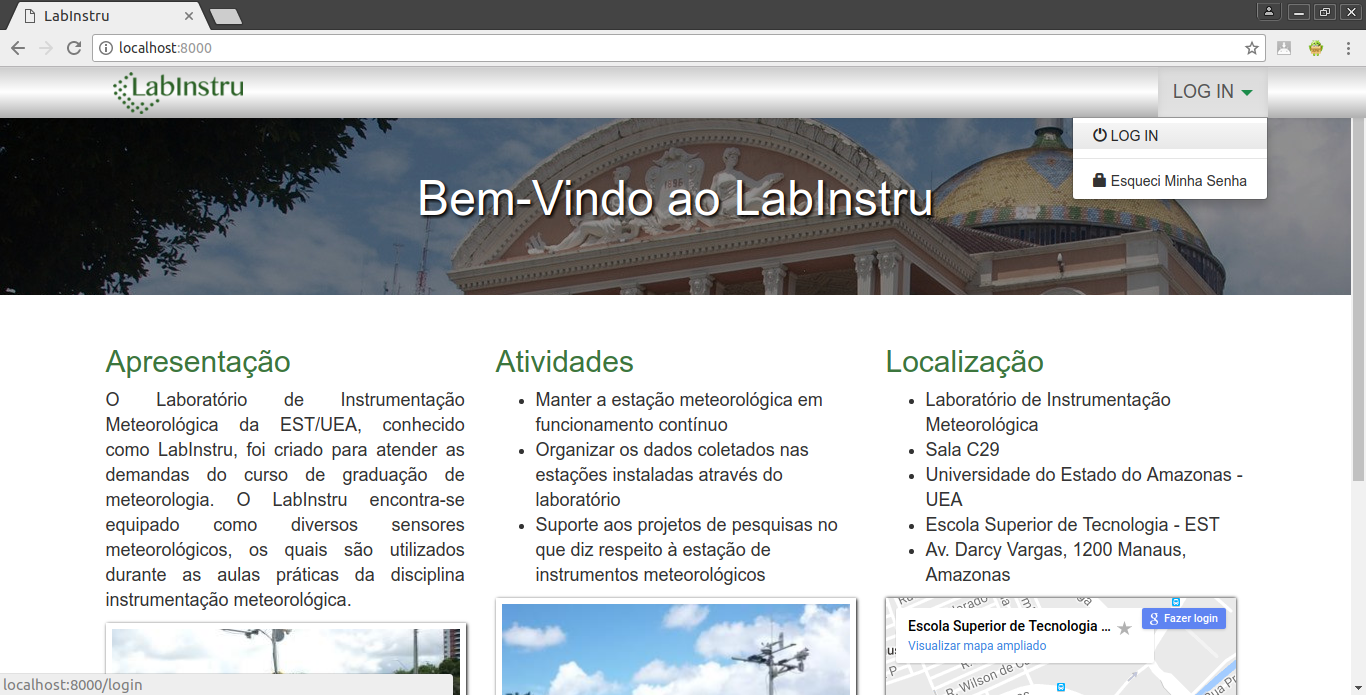
\includegraphics[width=0.9\textwidth]{./img/ap1.png}
	\caption{Página inicial da aplicação LabInstru Web. Fonte: Próprio autor.} \label{fig:ap1}
\end{figure}

\begin{figure}[h!]
	\centering
	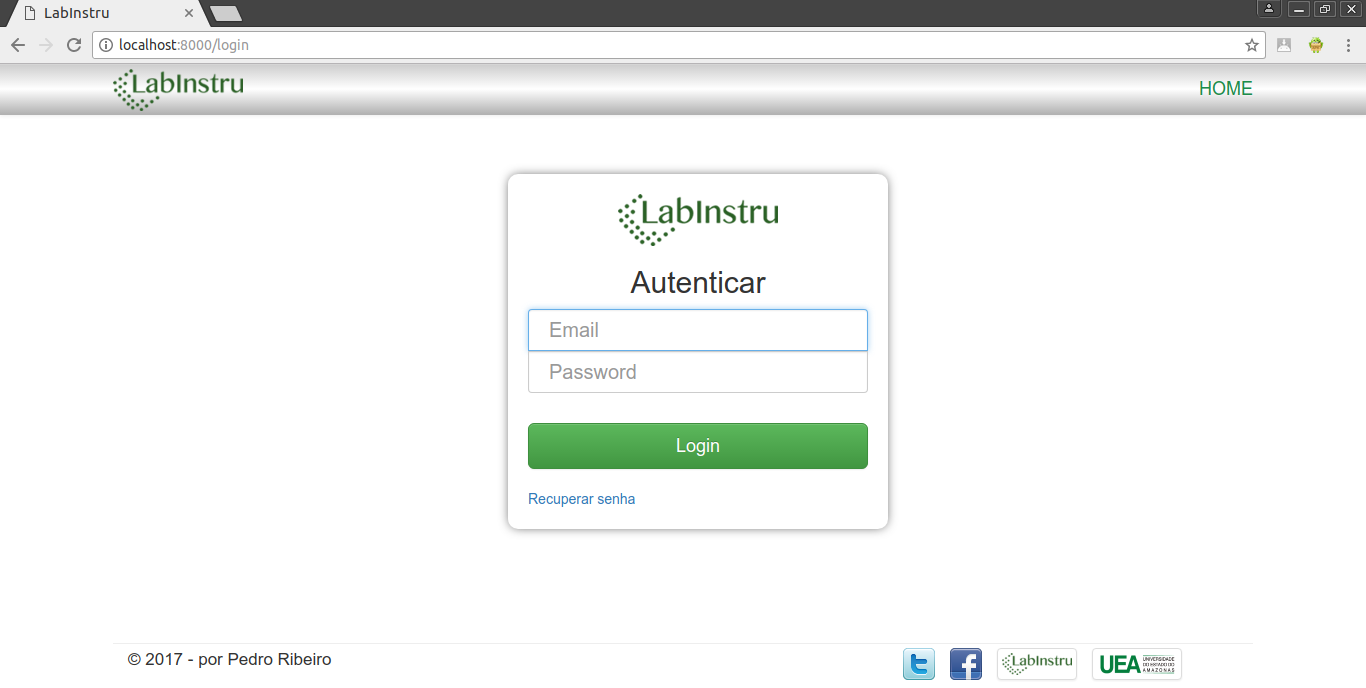
\includegraphics[width=0.9\textwidth]{./img/ap10.png}
	\caption{Formulário de autenticação do sistema. Fonte: Próprio autor.} \label{fig:ap10}
\end{figure}



\begin{figure}[h!]
	\centering
	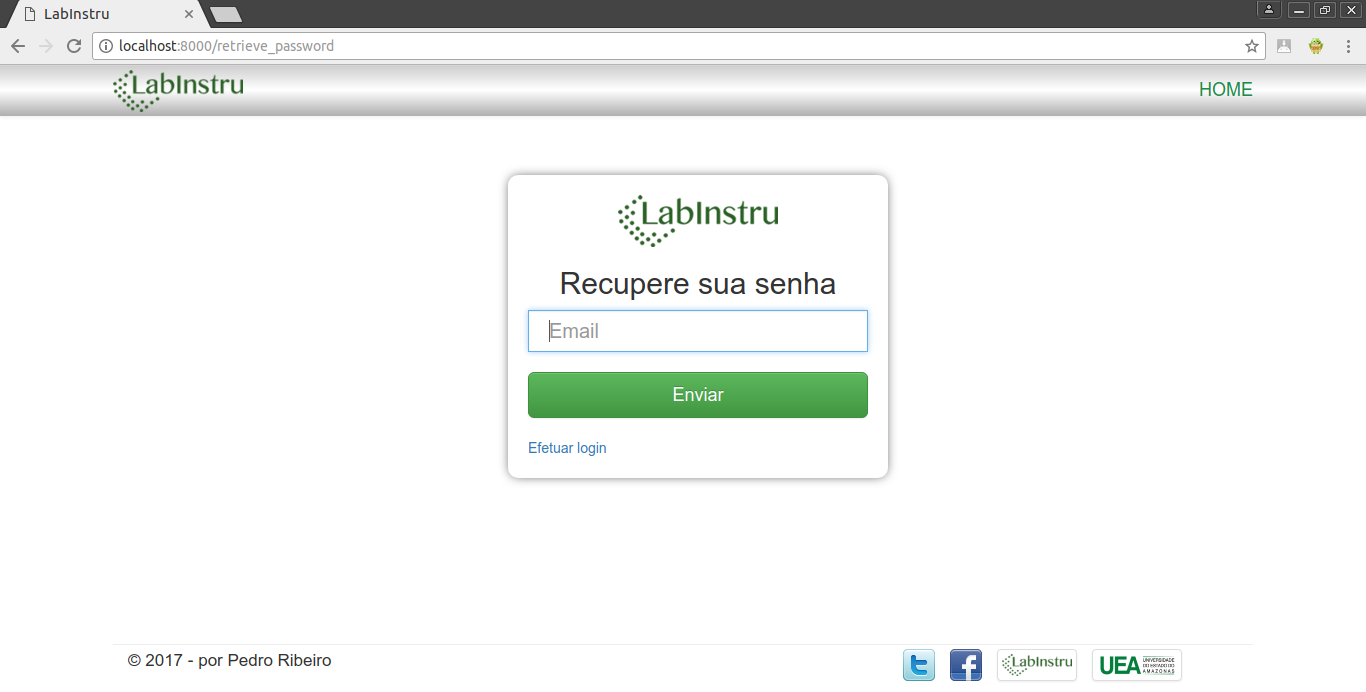
\includegraphics[width=0.9\textwidth]{./img/ap11.png}
	\caption{Formulário para recuperação de senha. Fonte: Próprio autor} \label{fig:ap11}
\end{figure}

A plataforma contempla dois perfis diferentes de acesso: um administrador, a ser desempenhado em termos práticos pela Profa. Maria Betânia Leal, responsável pelo LabInstru, e diversos usuários. O administrador, em especial, é o responsável por fornecer como entrada os dados advindos da estação meteorológica da EST para o LabInstru Web, conforme ilustrado na Figura \ref{fig:ap12}. A aplicação, após processar e persistir os dados advindos da estação, irá fornecer um sumário a respeito do status desta inserção, sob a forma de um \emph{log}. Este \emph{log} exibe quantas medições possuía o arquivo fornecido como entrada, quantas foram corretamente persistidas e quantas resultaram em falha. Um exemplo deste \emph{log} produzido pela aplicação é mostrado na Figura \ref{fig:ap13}.

\begin{figure}[h!]
	\centering
	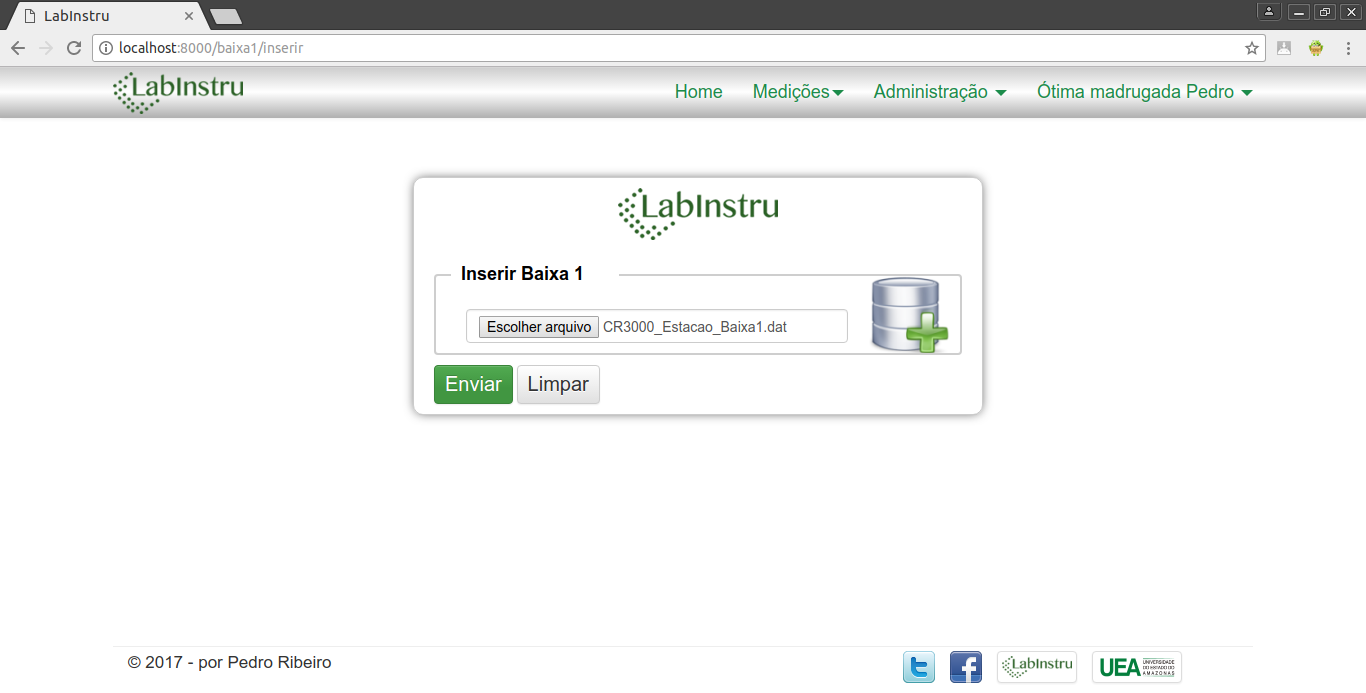
\includegraphics[width=0.9\textwidth]{./img/ap12.png}
	\caption{Página que disponibiliza o formulário para inserção de medições. Fonte: Próprio autor} \label{fig:ap12}
\end{figure}

\begin{figure}[h!]
	\centering
	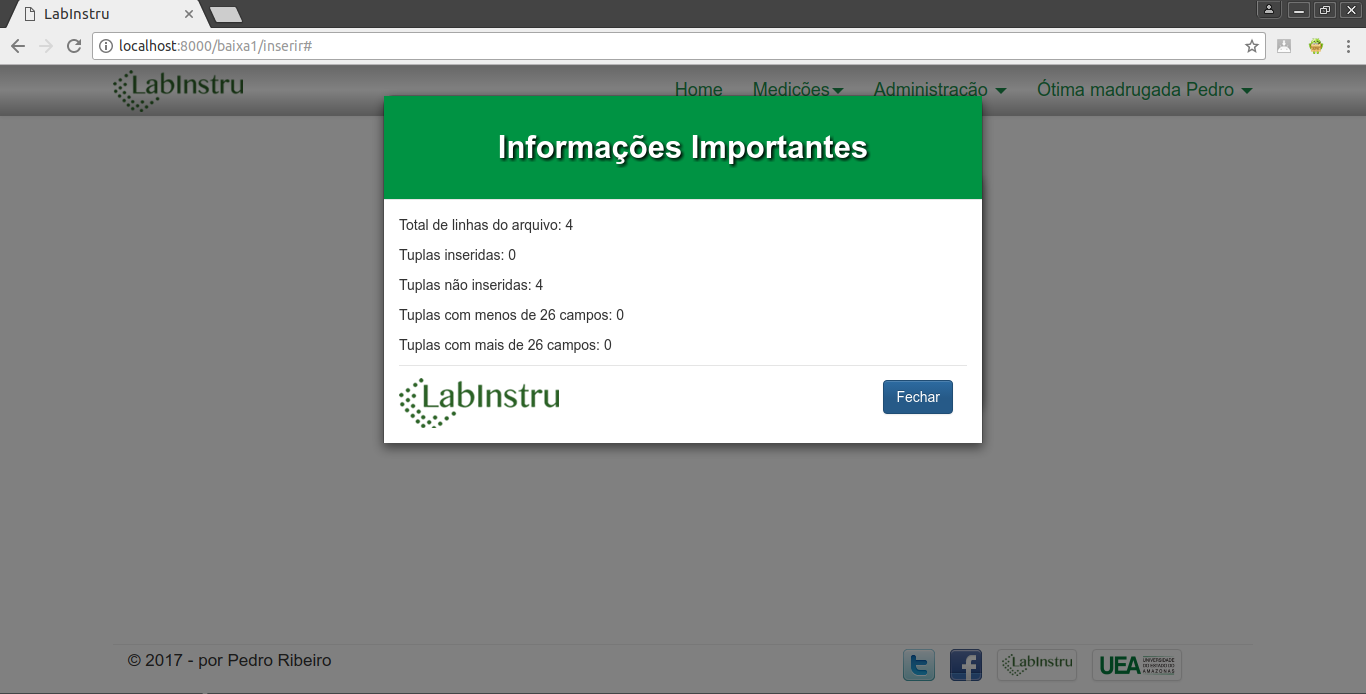
\includegraphics[width=0.9\textwidth]{./img/ap13.png}
	\caption{Exemplo de \emph{log} informando o resultado de uma inserção de medições. Fonte: Próprio autor} \label{fig:ap13}
\end{figure}



O administrador também fica responsável por cadastrar usuários, vide Figura \ref{fig:ap4}, que podem ser alunos de graduação e pós-graduação, outros pesquisadores, docentes, etc. Cabe também ao administrador da aplicação, por meio de uma listagem de usuários disponibilizada pela aplicação, realizar o gerenciamento dos usuários cadastrados na aplicação, conforme ilustrado na Figura \ref{fig:ap14}.

\begin{figure}[h!]
	\centering
	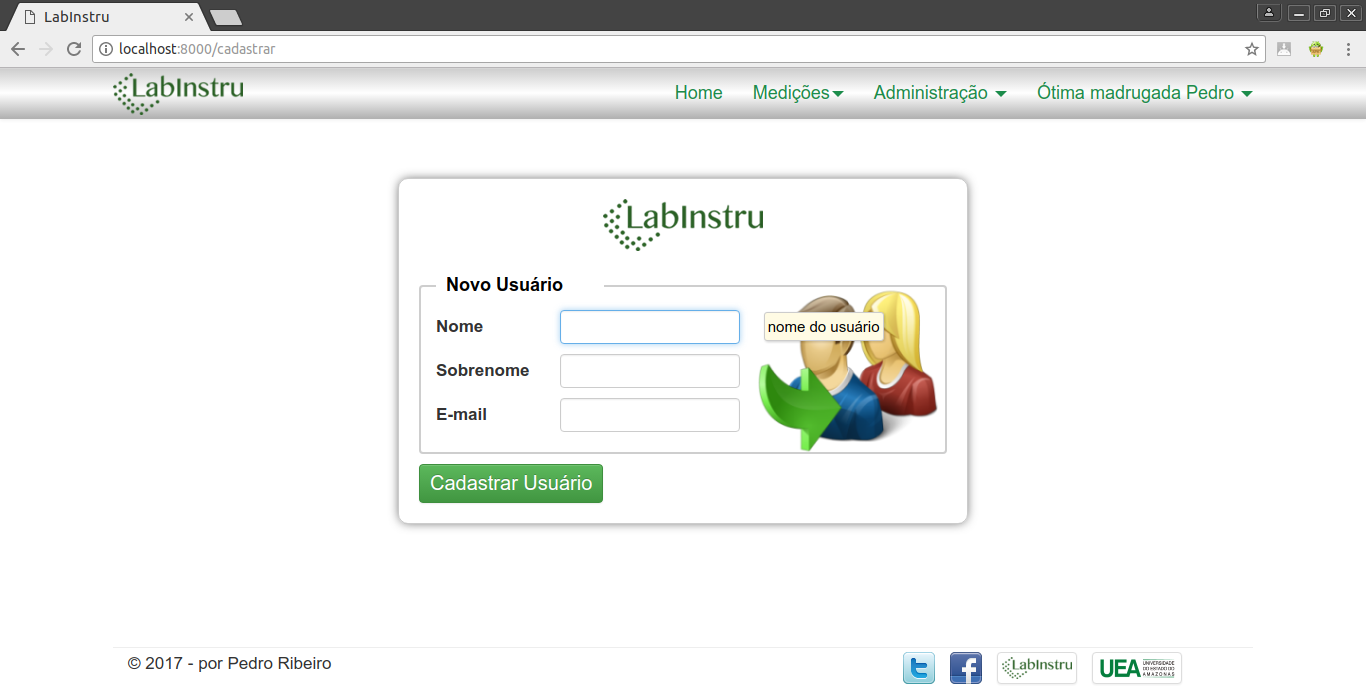
\includegraphics[width=0.9\textwidth]{./img/ap4.png}
	\caption{Página de cadastrado de usuário na plataforma LabInstru Web. Fonte: Próprio autor.} \label{fig:ap4}
\end{figure}

\begin{figure}[h!]
	\centering
	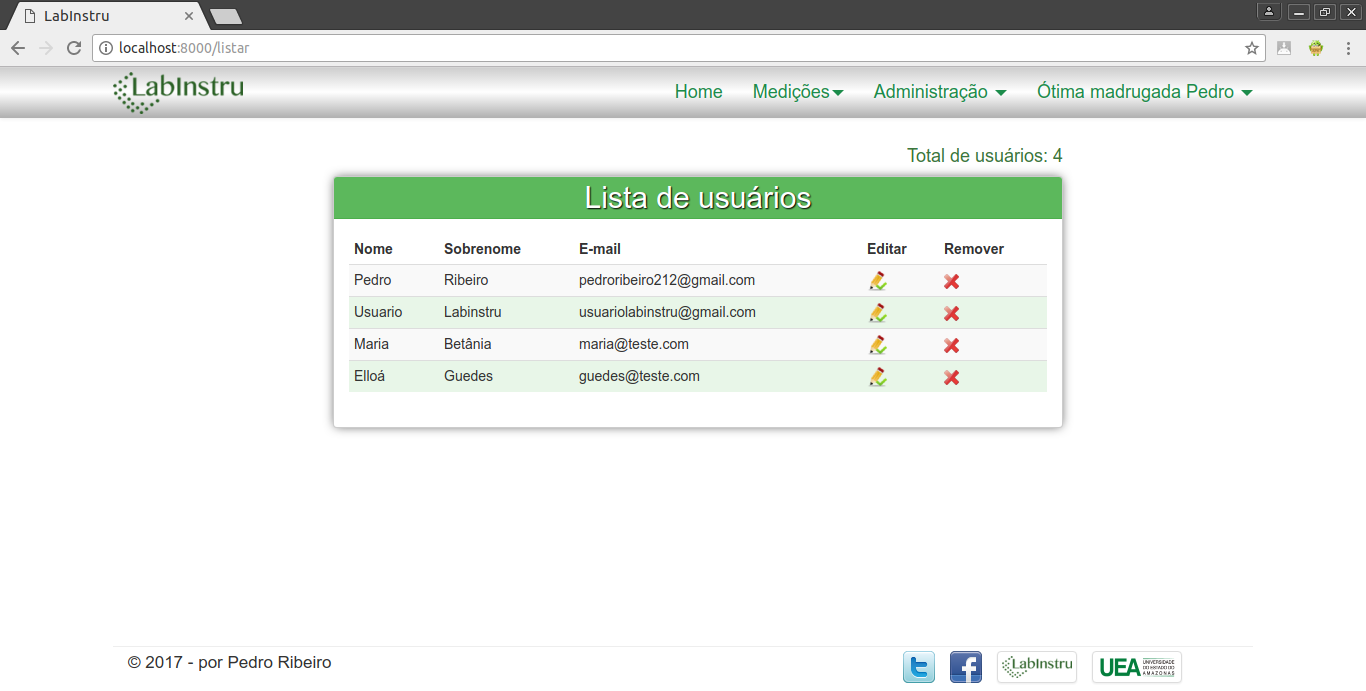
\includegraphics[width=0.9\textwidth]{./img/ap14.png}
	\caption{Lista de usuários cadastrados na aplicação. Fonte: Próprio autor.} \label{fig:ap14}
\end{figure}

Um menu superior, mostrado na Figura \ref{fig:ap1}, permite a autenticação dos usuários e também mostra as principais funcionalidades disponíveis na plataforma após realizada autenticação no sistema. Este menu é renderizado conforme o perfil do usuário. Por exemplo, o menu mostrado ao administrador dispõe da funcionalidade de apagar medições, funcionalidade não disponível no menu mostrado a um usuário. Os menus correspondentes aos diferentes perfis de usuário são ilustrados na Figura \ref{fig:ap8}. Ressalta-se que, independentemente do tipo do perfil de usuário, as principais funcionalidades da plataforma só poderão ser acessadas mediante prévia autenticação na plataforma via login e senha.

\todo{Nova versão da figura, refletindo o novo menu}
\begin{figure}[h!]
	\centering
	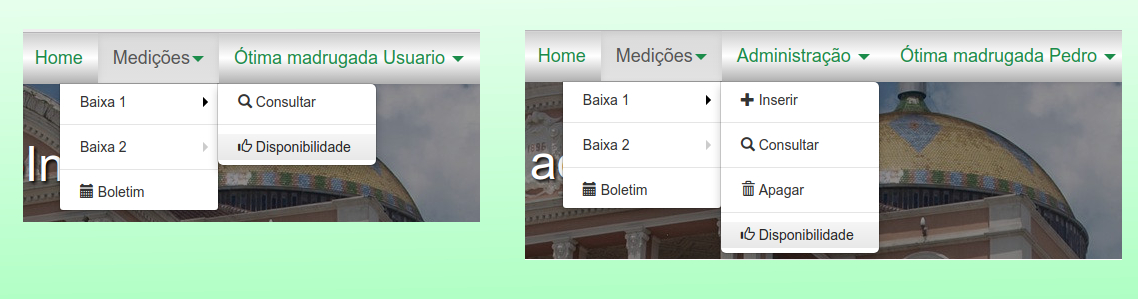
\includegraphics[width=0.9\textwidth]{./img/ap8.png}
	\caption{Exemplos dos menus para diferentes perfis de usuário. Fonte: Próprio autor.} \label{fig:ap8}
\end{figure}

As funcionalidades que permitem a mudança de senha e alteração de seus dados cadastrais são comuns aos dois perfis de usuários. Para ter acesso as mesmas, é necessário apenas que o usuário ou administrador encontre-se autenticado na aplicação. As Figuras \ref{fig:ap5} e \ref{fig:ap6} ilustram, respectivamente, os formulários para mudança de senha e alteração dos dados cadastrais de um determinado usuário (perfil).

\begin{figure}[h!]
	\centering
	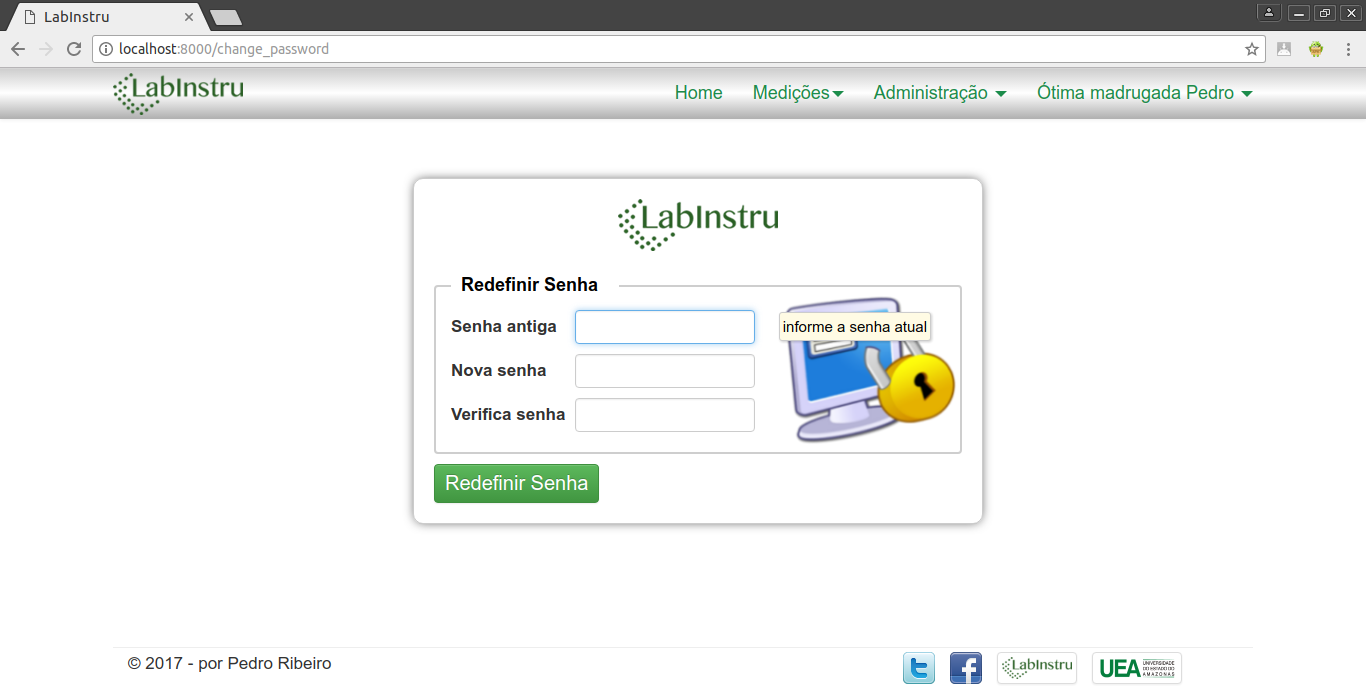
\includegraphics[width=0.9\textwidth]{./img/ap5.png}
	\caption{Formulário para troca de senha. Fonte: Próprio autor.} \label{fig:ap5}
\end{figure}

\begin{figure}[h!]
	\centering
	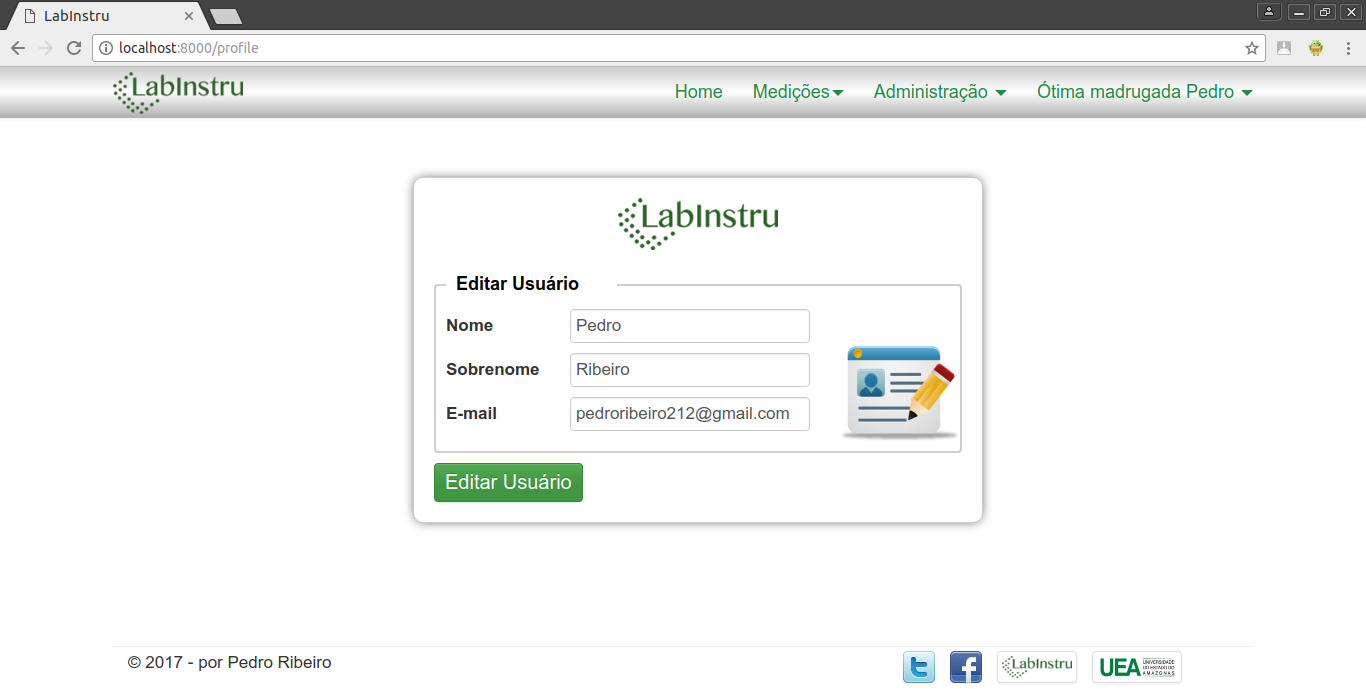
\includegraphics[width=0.9\textwidth]{./img/ap6.png}
	\caption{Página referente a edição de usuário. Fonte: Próprio autor.} \label{fig:ap6}
\end{figure}


Os usuários da plataforma \emph{LabInstru Web} acessam os dados da estação meteorológica da EST por meio de consultas, nas quais fornecem datas iniciais e finais e escolhem as variáveis de interesse, conforme ilustrado na Figura \ref{fig:ap3}. Considerou-se como uma restrição essencial para garantir a integridade e a confiabilidade dos dados que apenas o administrador seria responsável por cadastrá-los.

\todo{Atualizar esta figura}
\begin{figure}[h!]
	\centering
	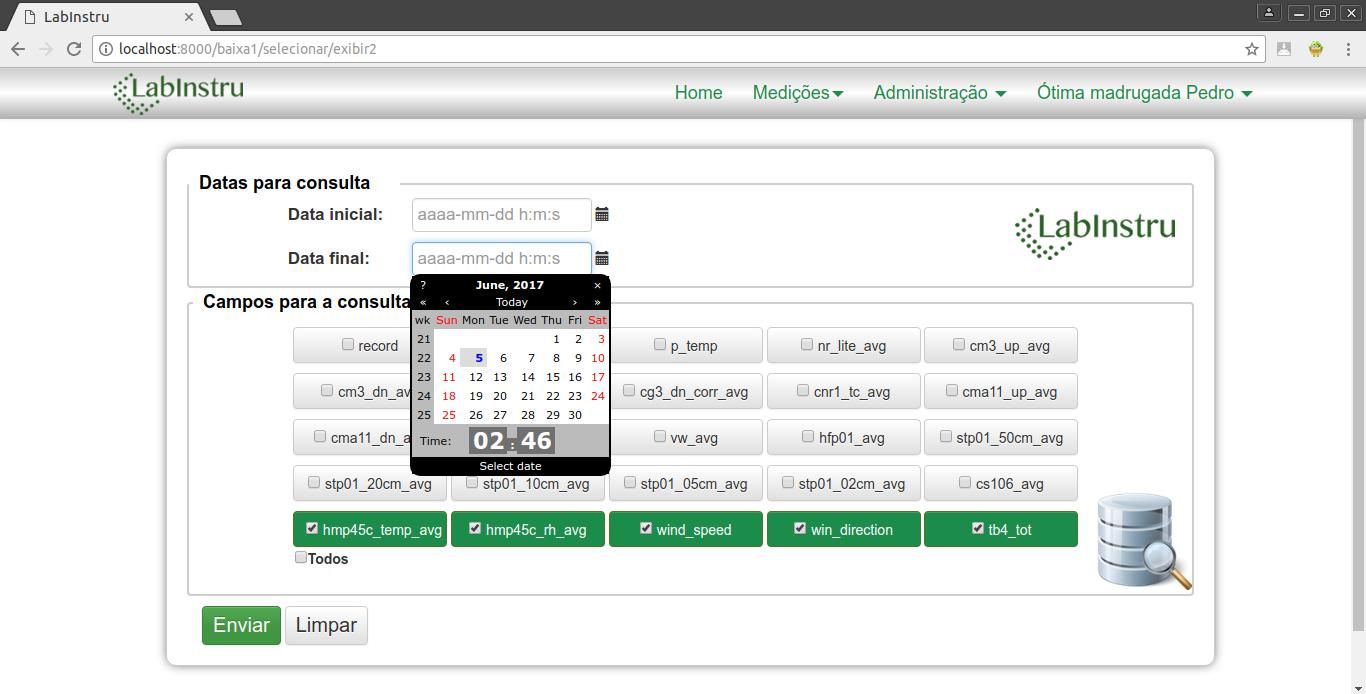
\includegraphics[width=0.9\textwidth]{./img/ap3.png}
	\caption{Página responsável por realizar as consultas. Fonte: Próprio Autor} \label{fig:ap3}
\end{figure}

Os resultados de uma consulta são exibidos em uma página apropriada, onde há opções para exportação dos mesmos nos formatos CSV, HTML, JSON, TSV e XML, conforme ilustra a Figura \ref{fig:ap7}.

\begin{figure}[h!]
	\centering
	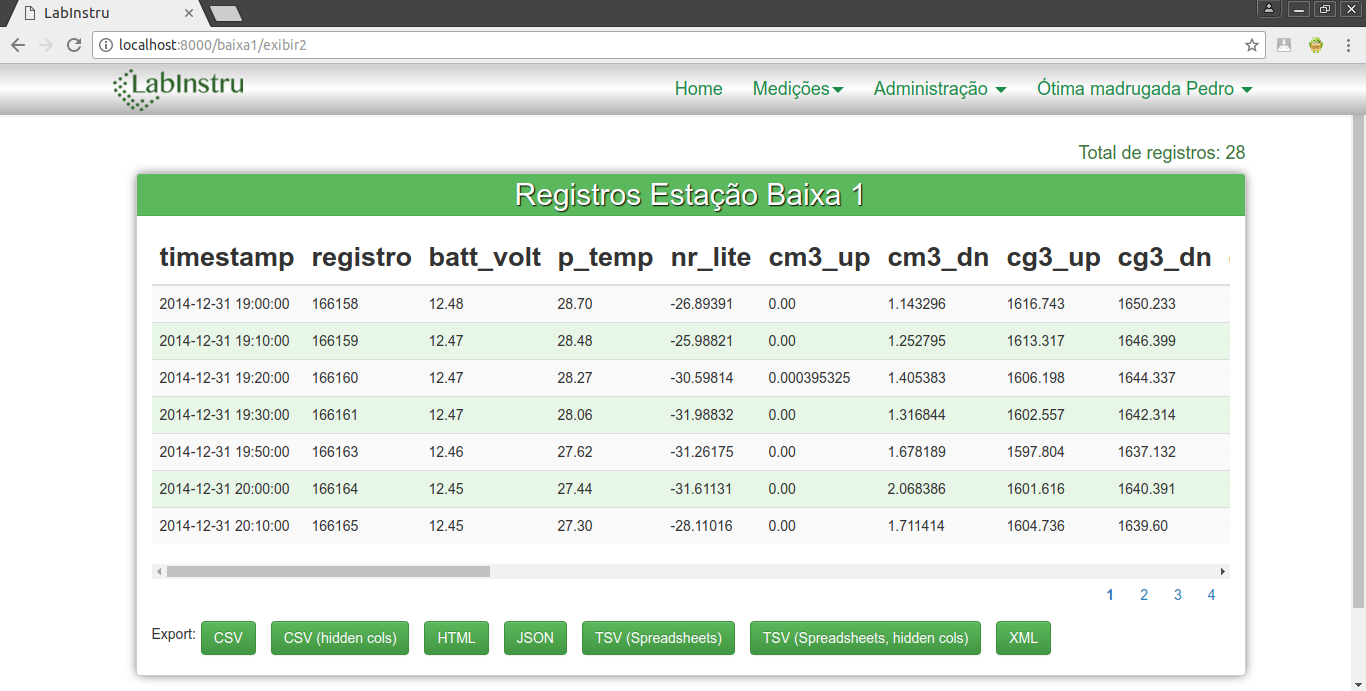
\includegraphics[width=0.9\textwidth]{./img/ap7.png}
	\caption{Página responsável por exibir o resultado de uma consulta. Fonte: Próprio Autor} \label{fig:ap7}
\end{figure}


\section{Modelo para Boletim Meteorológico}
Conforme identificado na elicitação de requisitos, uma das funcionalidades requeridas para a plataforma foi a geração de boletins meteorológicos diários, detalhados anteriormente na Seção \ref{sec:boletim}.

Para que esta funcionalidade fosse implementada adequadamente, um melhor refinamento de sua especificação foi necessário, visando a concepção do mesmo, da linguagem visual a ser adotada e dos elementos que deveriam ser incluídos. Como resultado, obteve-se o modelo apresentado na Figura \ref{fig:modeloBoletim}, que contempla a data, precipitação, temperaturas máxima e mínima, índice de calor, rajada e sua classificação na Escala de Beaufort, e ainda a logomarca do LabInstru e da Universidade do Estado do Amazonas.

\begin{figure}[h!]
	\centering
	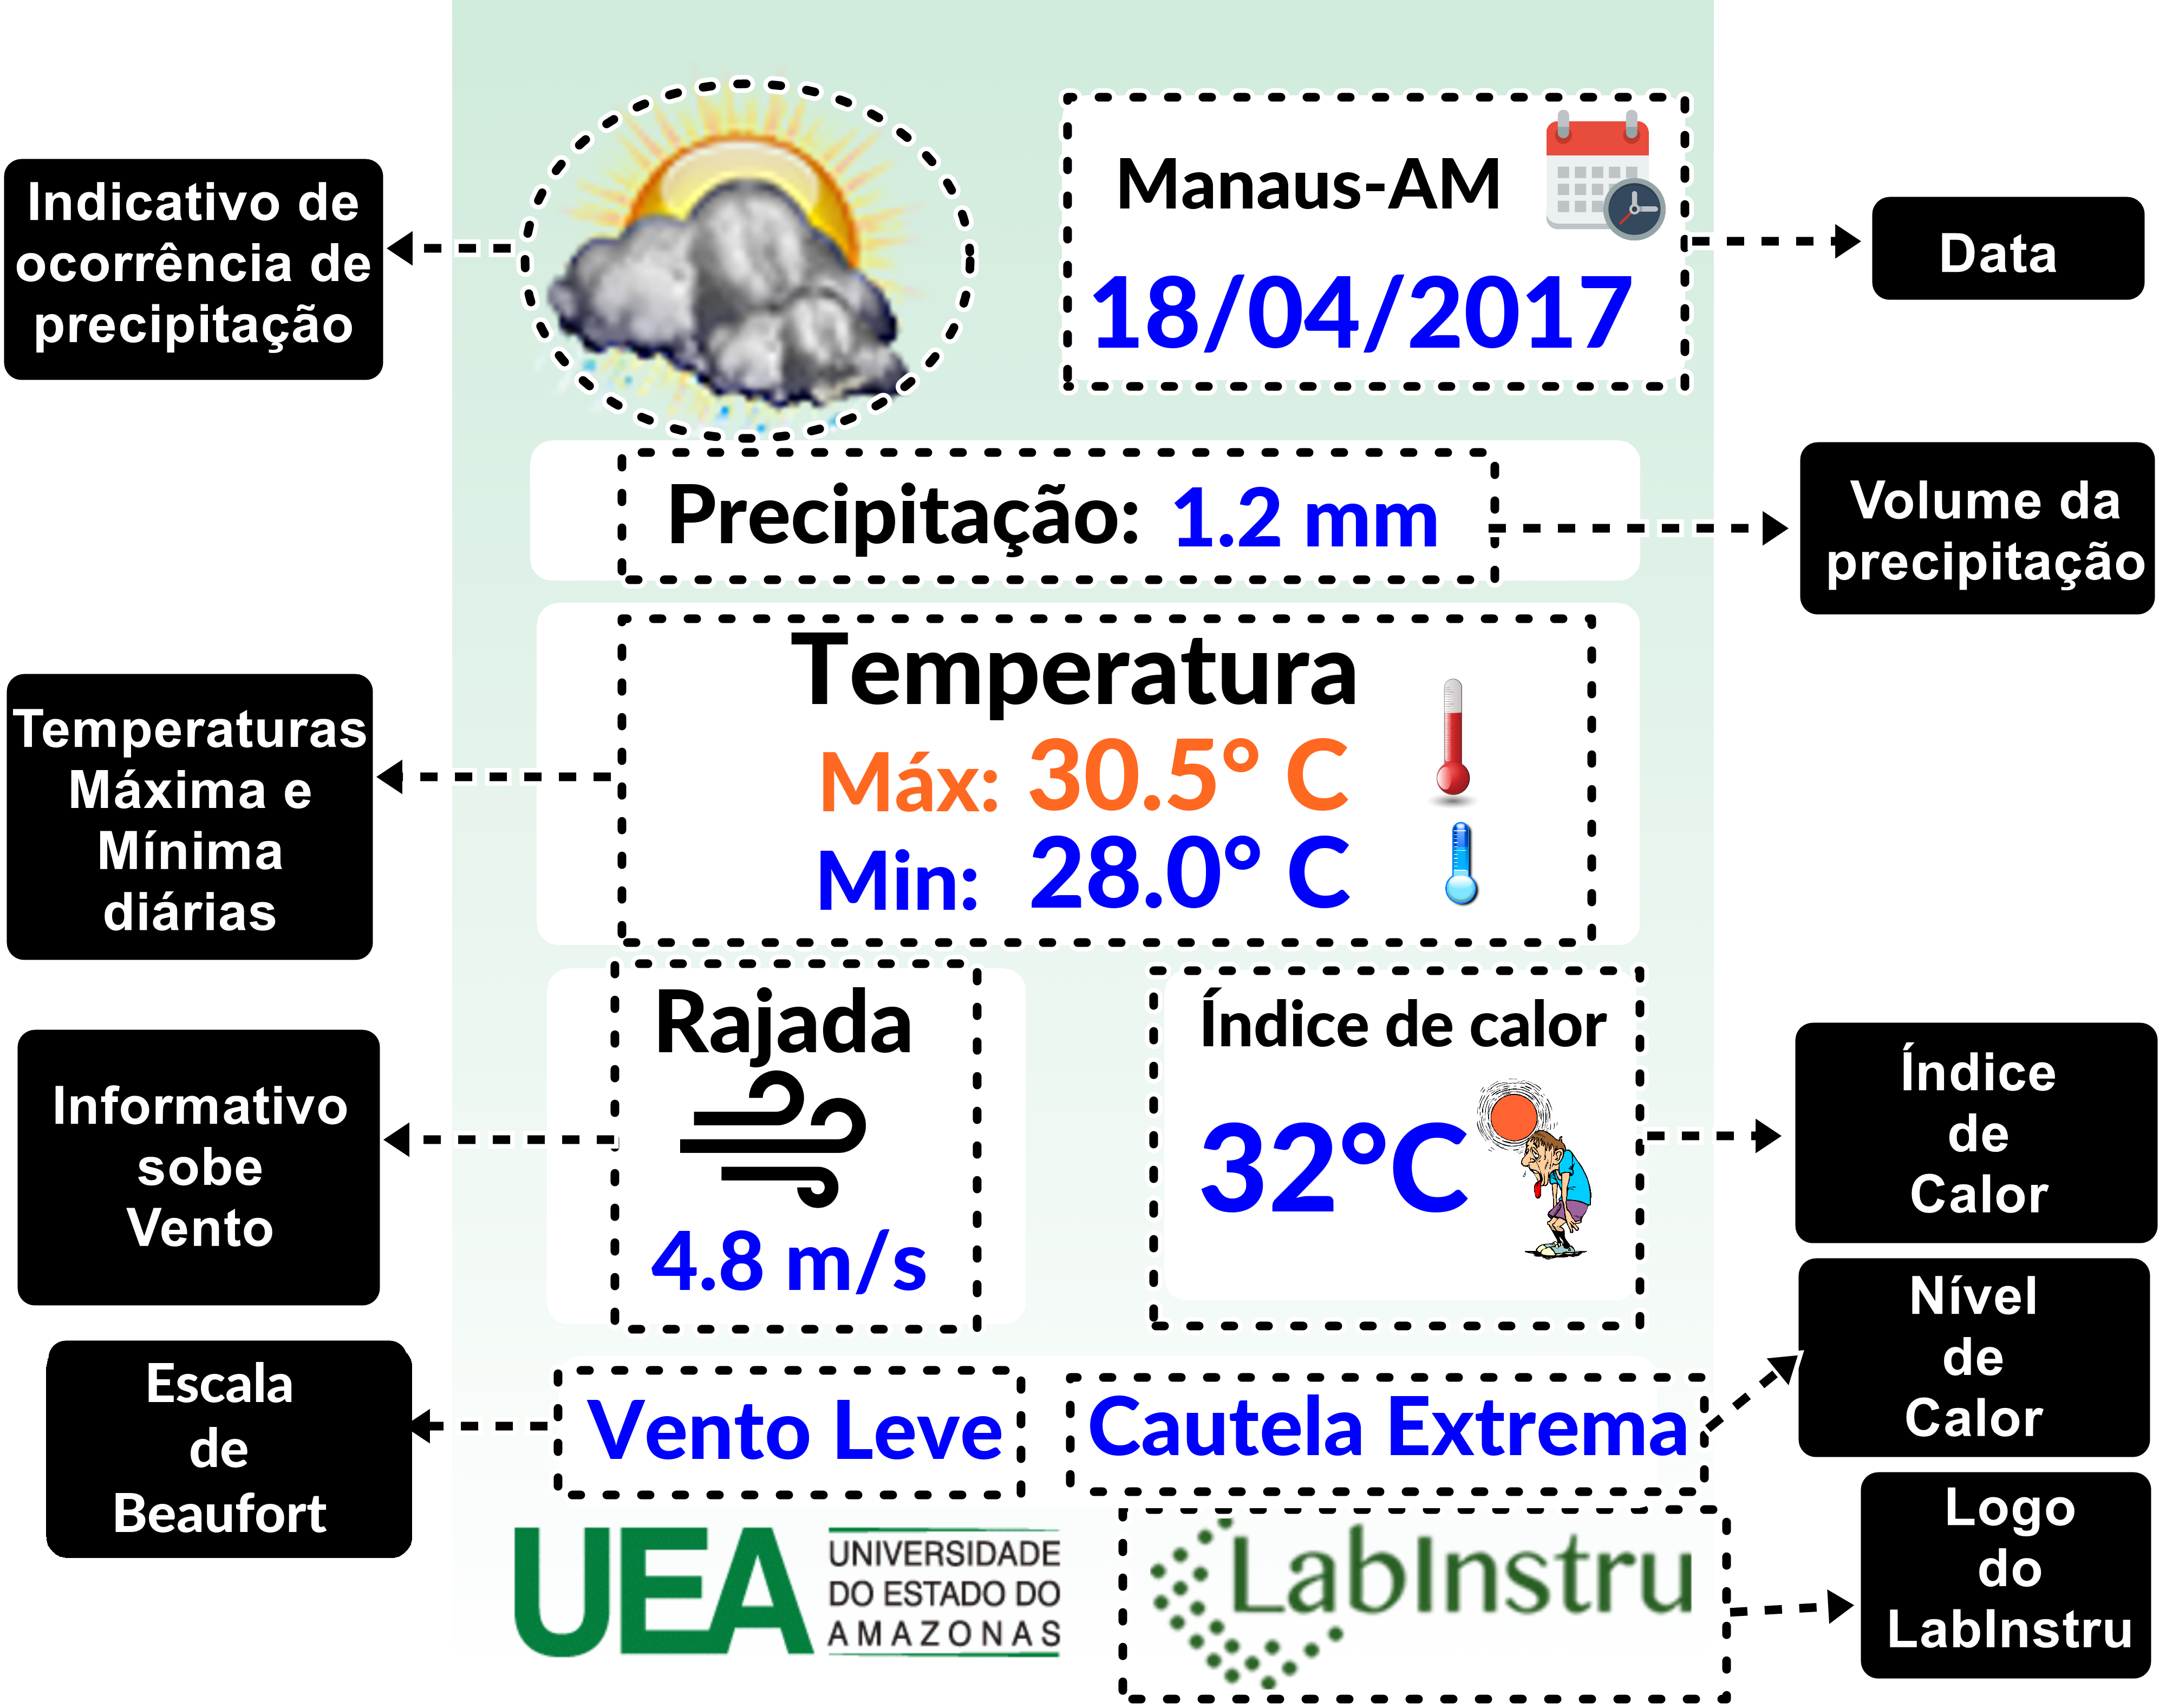
\includegraphics[width=0.5\textwidth]{./img/esbocoBoletim.png}
	\caption{Modelo de referência para boletim meteorológico. Fonte: Próprio autor.} \label{fig:modeloBoletim}
\end{figure}

Para automatizar a geração deste modelo de boletim na solução proposta, foi então necessário implementar o cálculo do índice de calor, desenvolver algoritmos para classificar a rajada e, principalmente, dedicar esforços na interface com o usuário para permitir uma visualização fiel ao modelo discutido com o cliente. Como resultado, o boletim meteorológico produzido com a solução proposta pode ser visto na Figura \ref{fig:boletim}.

\begin{figure}[h!]
	\centering
	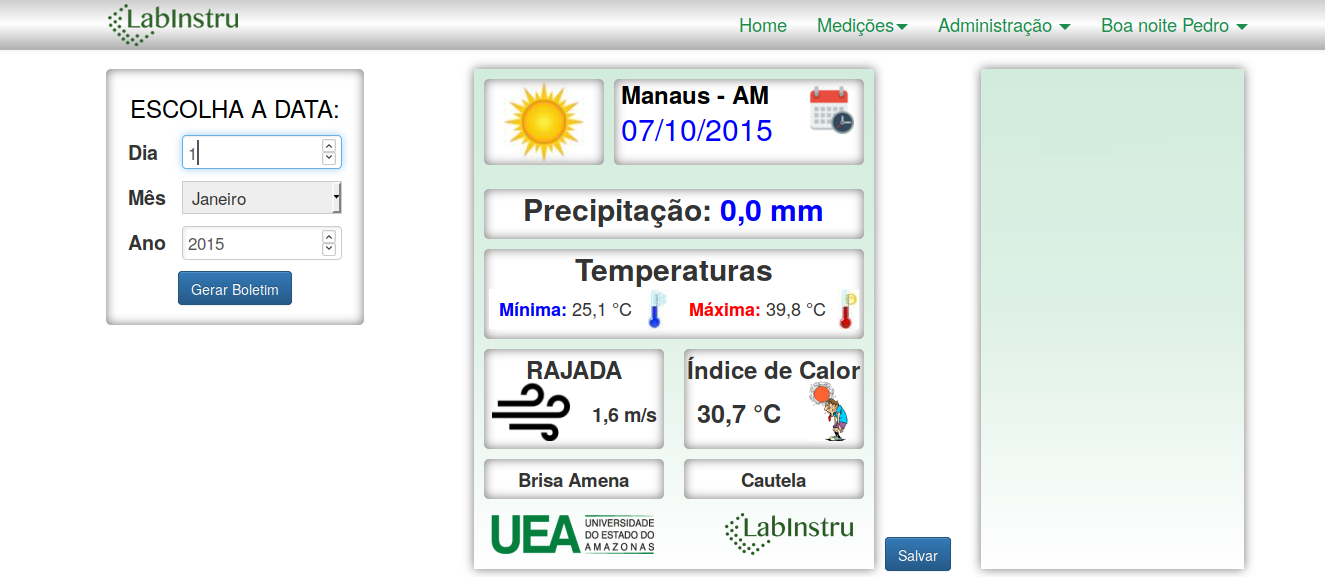
\includegraphics[width=0.9\textwidth]{./img/boletim.png}
	\caption{Boletim meteorológico produzido pelo LabInstru Web. Fonte: Próprio autor.} \label{fig:boletim}
\end{figure}


\chapter{Considerações Finais}

Este trabalho, por meio do desenvolvimento de uma aplicação web denominada LabInstru Web, colabora na minimização dos problemas enfrentados pelos pesquisadores do LabInstru na realização das atribuições deste laboratório. Considerando o tempo disponível, a existência de um único desenvolvedor e a possibilidade do surgimento de novos requisitos a qualquer momento, o Processo Ágil Unificado é o processo de desenvolvimento que tem guiado as disciplinas que levaram ao desenvolvimento da aplicação até o seu estágio atual.

Na implementação do LabInstru Web foi utilizado o \emph{framework} Web2py como base para o desenvolvimento da aplicação. Para o \emph{front-end} as tecnologias ágeis JQuery e Bootstrap colaboraram para produzir resultados mais visualmente agradáveis junto aos usuários.  Quanto ao \emph{back-end}, o sistema gerenciador de banco de dados MySQL foi utilizado para persistência dos dados por prover um bom desempenho na manipulação de uma quantidade significativa de dados.

Tão logo as funcionalidades remanescentes sejam implementadas, almeja-se que, após a implantação, o LabInstru Web proporcione benefícios aos pesquisadores do LabInstru, auxiliando-os a organizarem os dados da estação meteorológica da EST, permitindo que possam consultar estes dados para suas pesquisas (iniciação científica, mestrado, doutorado, etc.) de maneira mais rápida e eficiente e colaborando com a divulgação dos dados junto à população em geral por meio de boletins meteorológicos.

O desenvolvimento deste trabalho de conclusão de curso tem proporcionado a aplicação de conhecimentos obtidos nas disciplinas da grade do curso de Engenharia da Computação com vistas a resolver um problema real de um laboratório de instrumentação meteorológica. Disciplinas como Engenharia de Software, Banco de Dados e Linguagem de Programação foram cruciais para o desenvolvimento do mesmo. Entretanto, alguns conhecimentos tiveram de ser adquiridos de maneira independente, a exemplo do \emph{framework} considerado no desenvolvimento da aplicação web aqui proposta.
%\chapter{Exemplo}

\section{Tabela com o Pacote Booktabs}

Um exemplo de tabela com o pacote booktabs pode ser visto na Tabela \ref{tabela:exemplo}. A explica��o das tabelas sempre vem em cima e esse padr�o deve ser respeitado. A numera��o � autom�tica e a inser��o no �ndice tamb�m. Legal n�? \cite{Bennett:QuantumInformationSurvey}

Basta quebrar uma linha para criar um novo par�grafo. Neste par�grafo vou contar que tabelas no \LaTeX d�o um pouco de trabalho, mas nada que com paci�ncia n�o se resolva. Veja os links com dicas que coloquei nos coment�rios do arquivo \texttt{index.tex}.

\begin{table}[ht!]
\caption{Esta � uma tabela b�sica em \LaTeX com o pacote booktabs.} \label{tabela:exemplo}
\center{
\begin{tabular}{cccc}
\toprule
Parte 1 & Parte 2 & Parte 3 & Parte 4\\
\midrule
0,415 & 1,365 & 1,98 & 2,05\\
1,36  & 45,5  & 7,98 & 3,01\\
2,36  & 1,35  & 0,15 & 5,32\\
\bottomrule
\end{tabular}}
\end{table}



\section{Inser��o de Figuras}

Voc� pode inserir figuras JPG no \LaTeX! Veja o caso da Figura \ref{fig:exemplo}. Se voc� quiser outras configura��es e dicas, veja o seguinte endere�o: \url{http://en.wikibooks.org/wiki/LaTeX/Floats,_Figures_and_Captions}.

A explica��o da figura sempre vem embaixo da mesma. Isto aqui � um novo par�grafo apenas para ilustrar a id�ia geral de como escrever.

\begin{figure}[H]
\centering
\caption{Um exemplo de figura JPG inserida no \LaTeX.} \label{fig:exemplo}
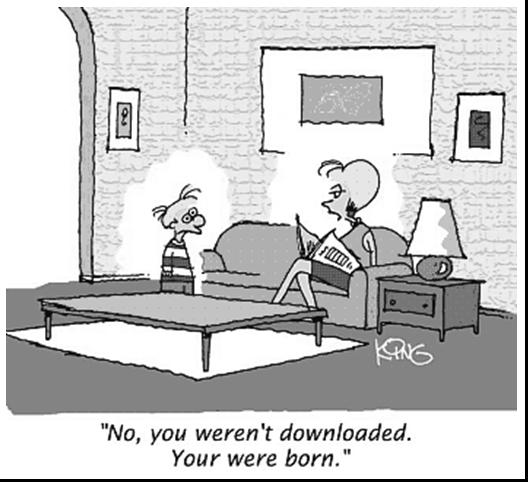
\includegraphics[width=0.4\textwidth]{./img/exemplo.jpg}\\
\small{Elaborado pelo autor.}
\end{figure}

Pode inserir v�rias figuras lado a lado tamb�m. Um exemplo est� reproduzido a seguir.

\begin{figure}[H]
  \centering
  \caption{Canal cl�ssico cuja obten��o da capacidade erro-zero � n�o-trivial.}
  \subfloat[\ ]{\label{fig:exG5}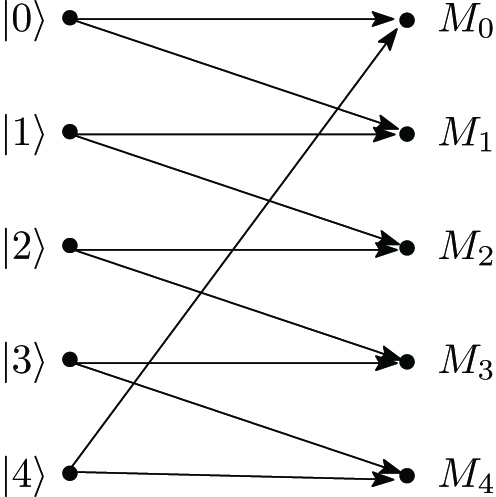
\includegraphics[width=0.3\textwidth]{./img/001}}
  \hspace{0.5cm}
  \subfloat[\ ]{\label{fig:exG52}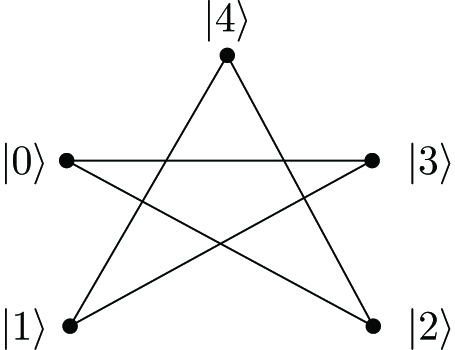
\includegraphics[width=0.3\textwidth]{./img/002}}
  \hspace{0.5cm}
  \subfloat[\ ]{\label{fig:exG53}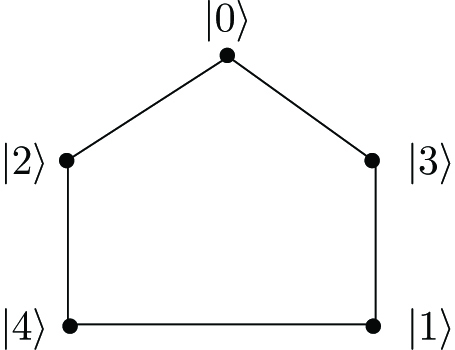
\includegraphics[width=0.3\textwidth]{./img/003}}\\
  \small{Elaborado por Bacon}
\end{figure}





\section{Refer�ncias Bibliogr�ficas no Padr�o ABNT}


%\chapter{T�tulo do Quarto Cap�tulo}


Vivamus ultricies tincidunt lacus ut pharetra. Sed fringilla hendrerit tempus. Suspendisse potenti. Cras hendrerit tortor ac est condimentum pellentesque. Morbi pretium lectus nec sapien laoreet eu malesuada diam adipiscing. Aliquam nisl ipsum, fermentum ut aliquam nec, varius sit amet nisi. Pellentesque interdum cursus malesuada. Vestibulum ante ipsum primis in faucibus orci luctus et ultrices posuere cubilia Curae; Nullam malesuada bibendum tortor, ut bibendum lorem varius eu. In eros orci, volutpat ut facilisis sit amet, commodo quis nulla.

Sed lectus metus, mollis nec vulputate id, imperdiet eget urna. Nam ut dolor at metus venenatis suscipit et in ligula. In hac habitasse platea dictumst. Mauris scelerisque dolor sed nisl mattis accumsan. Aliquam vulputate placerat feugiat. Pellentesque faucibus neque mi. Etiam porttitor varius tempus. Mauris varius porttitor posuere. Pellentesque iaculis imperdiet lobortis. Sed vulputate purus nec felis rutrum molestie.


\section{Algoritmos}




Nunc at fringilla dui. Pellentesque id tortor eu libero auctor rhoncus id vel velit. Duis auctor laoreet turpis, sed commodo tellus sollicitudin sit amet. Phasellus quis purus consectetur turpis hendrerit pretium eget in velit. Cras dignissim est vel mi malesuada a imperdiet velit condimentum. Vivamus ultrices diam non urna aliquet hendrerit. Sed lobortis, mauris quis egestas ullamcorper, nunc nulla auctor nulla, eu rutrum velit velit in nulla. Etiam lectus augue, pellentesque et porta at, pharetra id lectus. Duis eleifend eleifend mauris, nec mollis mauris vehicula nec. Nam sed ipsum ut massa lacinia vestibulum. Duis vitae sapien a lectus aliquam luctus eget sit amet nunc. Etiam a ipsum auctor tortor condimentum consectetur. Aliquam vestibulum libero sit amet nulla auctor aliquet. Sed laoreet imperdiet tellus non vulputate. Vivamus tristique ipsum vel metus venenatis in laoreet tortor hendrerit. Suspendisse potenti. Aenean tincidunt molestie libero sit amet porttitor. Class aptent taciti sociosqu ad litora torquent per conubia nostra, per inceptos himenaeos.





Cras nec quam mi, ut mattis ante. Lorem ipsum dolor sit amet, consectetur adipiscing elit. Sed fringilla auctor dictum. Nam hendrerit sapien sed massa consequat rutrum. Nullam congue, augue sed commodo malesuada, lectus nulla mollis magna, eget semper risus nisl eget elit. Duis vitae hendrerit massa. In a odio nunc, sit amet mollis dolor. In accumsan suscipit dui, a vestibulum diam condimentum ullamcorper. Etiam ut quam arcu, ac tristique ante. Vestibulum imperdiet elit non ante tristique accumsan. Donec vulputate fringilla tempor. Proin porttitor nisi nisi. Fusce vel ullamcorper orci. Lorem ipsum dolor sit amet, consectetur adipiscing elit. 

Vivamus ultricies tincidunt lacus ut pharetra. Sed fringilla hendrerit tempus. Suspendisse potenti. Cras hendrerit tortor ac est condimentum pellentesque. Morbi pretium lectus nec sapien laoreet eu malesuada diam adipiscing. Aliquam nisl ipsum, fermentum ut aliquam nec, varius sit amet nisi. Pellentesque interdum cursus malesuada. Vestibulum ante ipsum primis in faucibus orci luctus et ultrices posuere cubilia Curae; Nullam malesuada bibendum tortor, ut bibendum lorem varius eu. In eros orci, volutpat ut facilisis sit amet, commodo quis nulla.





% Referência segundo o padrão ABNT
% Edite este arquivo e inclua suas referências segundo a notação do Bibtex
\bibliography{ref}



\end{document}